% Copyright (c) 2022 by Lars Spreng
% This work is licensed under the Creative Commons Attribution 4.0 International License. 
% To view a copy of this license, visit http://creativecommons.org/licenses/by/4.0/ or send a letter to Creative Commons, PO Box 1866, Mountain View, CA 94042, USA.

%~~~~~~~~~~~~~~~~~~~~~~~~~~~~~~~~~~~~~~~~~~~~~~~~~~~~~~~~~~~~~~~~~~~~~~~~~~~~~~
% You can add your packages and commands to the loadslides.tex file. 
% The files in the folder "styles" can be modified to change the layout and design of your slides.
% I have included examples on how to use the template below. 
% Some of these examples are taken from the Metropolis template.
%~~~~~~~~~~~~~~~~~~~~~~~~~~~~~~~~~~~~~~~~~~~~~~~~~~~~~~~~~~~~~~~~~~~~~~~~~~~~~~


\documentclass[
11pt,notheorems,hyperref={pdfauthor=whatever}
]{beamer}

\usepackage{amssymb}
% \input{template_macros.tex}
\usepackage{tcolorbox}
\usepackage{graphicx}
\usepackage{xcolor}
\renewcommand{\familydefault}{\sfdefault}
\usepackage{tikz}
\usepackage{tikz-3dplot}
\usetikzlibrary{positioning, arrows.meta, shapes.geometric, calc, backgrounds, fit}
% % Make slides black + default text white
% \setbeamercolor{background canvas}{bg=black}
% \setbeamercolor{normal text}{fg=white,bg=black}


\input{loadslides.tex} % Loads packages and some defined commands

\setbeamersize{
  text margin left=60mm,
  text margin right=10mm
}

% put these AFTER the theme/colors are loaded
\setbeamercolor{background canvas}{bg=black}
\setbeamercolor{normal text}{fg=white,bg=black}
\definecolor{accTeal}{RGB}{77, 208, 225}
\definecolor{accGreen}{RGB}{129, 199, 132}
\definecolor{accAmber}{RGB}{255, 213, 79}
\definecolor{accCoral}{RGB}{255, 138, 101}

\definecolor{bgTeal}{RGB}{15, 30, 40}
\definecolor{bgGreen}{RGB}{15, 30, 20}
\definecolor{bgAmber}{RGB}{30, 25, 10}
\definecolor{bgCoral}{RGB}{35, 15, 15}

\newcommand{\HUGE}{\fontsize{28pt}{32pt}\selectfont}
\setbeamercolor{alerted text}{fg=yellow!60}
\title[
% Text entered here will appear in the bottom middle
]{Medical Image Analysis Lectures}

% \subtitle{Presentation Subtitle}

% \author[
% % Text entered here will appear in the bottom left corner
% ]{
%     Tianyi Ren 
% }

\institute{
    Mehmet Kurt, Tianyi Ren \\
    University of Wasghinton}
\date{\today}

\begin{document}

% Generate title page
{
\setbeamertemplate{footline}{} 
\setbeamercolor{title}{fg=primary,bg=black}
\setbeamercolor{subtitle}{fg=secondary,bg=black}
\setbeamercolor{author}{fg=white,bg=black}
\setbeamercolor{institute}{fg=white,bg=black}
\setbeamercolor{date}{fg=white,bg=black}
\begin{frame}
  \titlepage
\end{frame}
}
\addtocounter{framenumber}{-1}
\definecolor{glassbg}{RGB}{255, 255, 255} % Base for transparency

\tcbset{
    medicalglass/.style={
        standard jigsaw,
        opacityback=0.08,    % High transparency
        opacityframe=0.4,    % Visible but subtle border
        colupper=white!95!blue, % "Ghost White" for body text
        coltitle=white,      % Pure white for titles
        fonttitle=\bfseries\large,
        arc=4pt,
        boxrule=1.2pt,
        left=6pt, right=6pt, top=4pt, bottom=4pt,
        before skip=6pt, after skip=6pt
    }
}



%%%%%%%%%%%%%%%%%%%%%%%%%%%%%%%%%%%%%%%%%%%%%%%%
%%%%%%%%%%%%%%%%%%%%%%%%%%%%%%%%%%%%%%%%%%%%%%%%

% You can declare different parts as a parentof sections
% \begin{frame}{Part I: Biomedical Image Applications}
%     \tableofcontents[part=1]
% \end{frame}
% \begin{frame}{Part II: History of Computer Vision}
%     \tableofcontents[part=2]
% \end{frame}


%%%%%%%%%%%%%%%%%%%%%%%%%%%%%%%%%%%%%%%%%%%%%%%%
%%%%%%%%%%%%%%%%%%%%%%%%%%%%%%%%%%%%%%%%%%%%%%%%


\makepart{Introduction to Medical image}



\begin{frame}{Imaging volume and complexity are increasing}
\small
%     \column{0.42\linewidth}
    \centering
    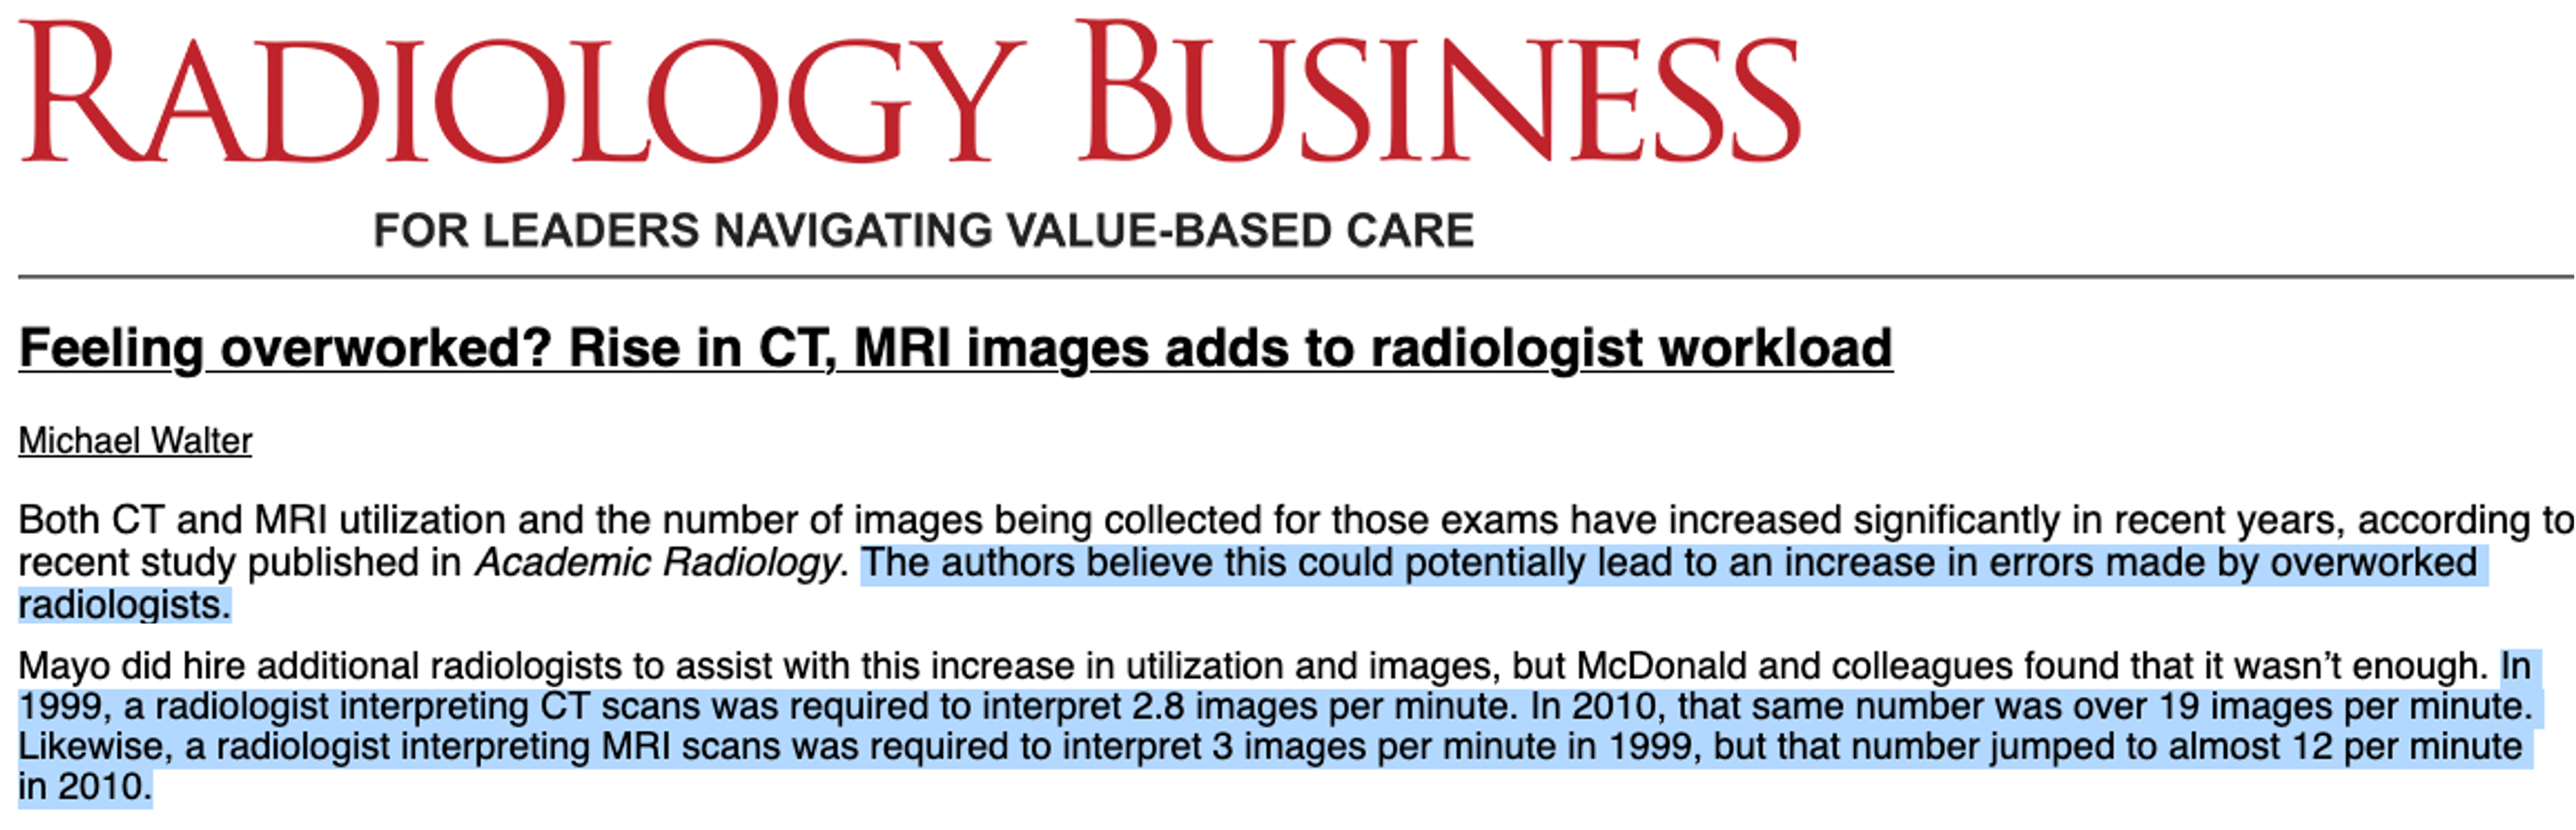
\includegraphics[width=1\linewidth]{Figures/radiology_bussiness.png}
\vfill
% \begin{flushleft}
% \tiny Source: \href{https://doi.org/10.1186/s13244-019-0832-5}{Lassau et al., Insights Imaging 2019}
% \end{flushleft}

\end{frame}



\begin{frame}{Medical Knowledge is highly subspecialized}

    
    \vspace{1cm}

    \begin{columns}[T]
        % Left Column: MRI and text
        \begin{column}{0.45\textwidth}
            \centering
            % Replace 'example-image-a' with your MRI file path
            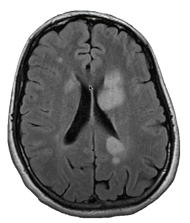
\includegraphics[width=0.6\linewidth]{Figures/glioma_example.png} 
            
            \vspace{0.5cm}
            \textbf{Glioma?}\\
            \textbf{ADEM?}\\
            \textbf{HIV encephalopathy?}
        \end{column}

        % Right Column: Rotated Journal Article
        \begin{column}{0.55\textwidth}
            \centering
            \vspace{1cm}
            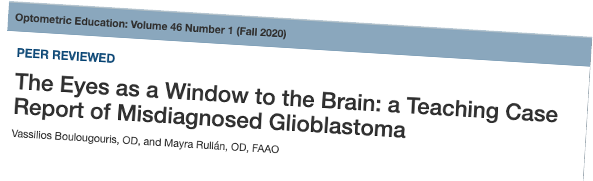
\includegraphics[width=1\linewidth, angle=-5]{Figures/news1.png}
        \end{column}
    \end{columns}
\end{frame}


\begin{frame}{Medical Knowledge is highly subspecialized}
    
    \vspace{1.5cm}

    \begin{columns}[T]
        % Left Column: MRI and text
        \begin{column}{0.45\textwidth}
            \centering
            % --- Placeholder for your brain MRI image ---
            % \includegraphics[width=0.6\linewidth]{Figures/brain_mri.png} 
            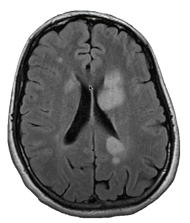
\includegraphics[width=0.6\linewidth]{Figures/glioma_example.png} % Example image, replace with your MRI file
            
            \vspace{0.8cm}
            \textbf{Glioma?}\\
            \textbf{ADEM?}\\
            \textbf{HIV encephalopathy?}
        \end{column}

        % Right Column: Piled Journal Articles using TikZ for precise layering
        \begin{column}{0.55\textwidth}
            % --- Container for stacked images ---
            \begin{tikzpicture}
                
                % 1. Bottom Image: "The Eyes as a Window..."
                % Replace 'example-image-b' with the path to your first news screenshot
                \node[anchor=south west, rotate=-5] (image1) at (0,0) {
                    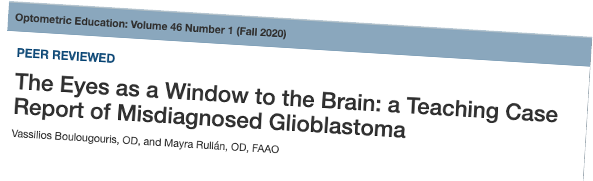
\includegraphics[width=1\linewidth]{Figures/news1.png} % replace with news1.png
                };
                
                \node[anchor=south west, rotate=+8] (image2) at (0.8, -1.0) {
                    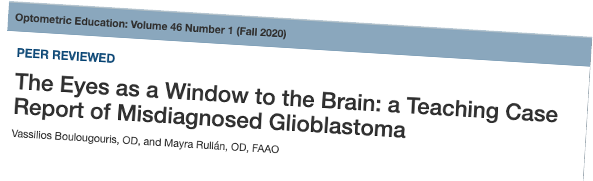
\includegraphics[width=1\linewidth]{Figures/news1.png} % replace with news2.png
                };
                
            \end{tikzpicture}
        \end{column}
    \end{columns}
\end{frame}


\begin{frame}{Medical Knowledge is highly subspecialized}
    
    \vspace{1cm}

    \begin{columns}[T]
        % Left Column: MRI and text
        \begin{column}{0.45\textwidth}
            \centering
            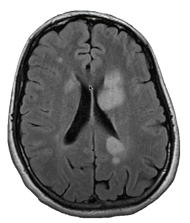
\includegraphics[width=0.65\linewidth]{Figures/glioma_example.png} 
            
            \vspace{0.6cm}
            \textbf{Glioma?}\\
            \textbf{ADEM?}\\
            \textbf{HIV encephalopathy?}
        \end{column}

        % Right Column: Three Stacked Journal Articles
        \begin{column}{0.55\textwidth}
            \centering
            \vspace{0.8cm}
            \begin{tikzpicture}
                % 1. Bottom Image
                \node[anchor=center, rotate=-5] (img1) at (0,0) {
                    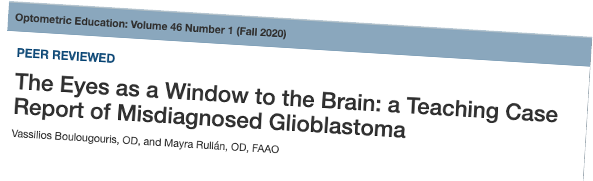
\includegraphics[width=1\linewidth]{Figures/news1.png}
                };
                
                % 2. Middle Image
                \node[anchor=center, rotate=+8] (img2) at (0.3,-0.5) {
                    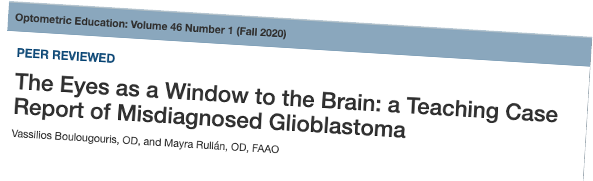
\includegraphics[width=1\linewidth]{Figures/news1.png}
                };
                
                % 3. Top Image (the most recent one you added)
                \node[anchor=center, rotate=-3] (img3) at (0.7,-1.1) {
                    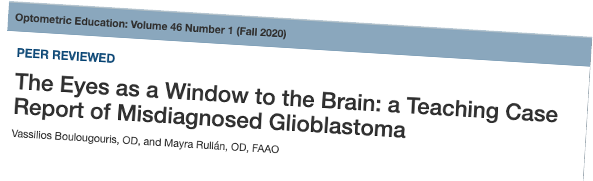
\includegraphics[width=1\linewidth]{Figures/news1.png}
                };
            \end{tikzpicture}
        \end{column}
    \end{columns}
\end{frame}


\begin{frame}{Trends in Medical AI Publications}
    \begin{itemize}
        \item Significant rise in scientific publications over the last decade
        \item Sharp increase in research output starting around 2016
    \end{itemize}

    \begin{figure}
        \centering
        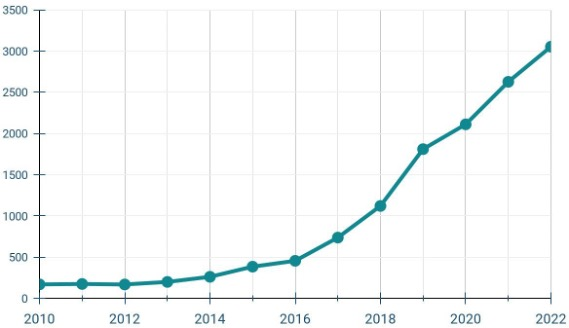
\includegraphics[width=0.75\textwidth]{Figures/numberofpapers.jpg}
        \caption{AI scientific publications in medical imaging}
    \end{figure}

    \vfill
    \footnotesize{Source: OECD AI 2022}
\end{frame}

%%%%%%%%%%%%%%%%%%%%%%%%%%%%%%%%%%%%%%%%%%%%%%%%
%%%%%%%%%%%%%%%%%%%%%%%%%%%%%%%%%%%%%%%%%%%%%%%%

\begin{frame}{Primary Modalities in Medical Imaging}
\centering

\begin{tikzpicture}[
    scale=0.4, transform shape, 
    font=\sffamily\color{white},
    phasebox/.style={
        rectangle, rounded corners=10pt, draw, thick,
        font=\sffamily\bfseries\Large\color{white},
        minimum width=9cm, 
        minimum height=16cm,
        align=center, 
        fill = black, 
        text width=7cm, 
        inner sep=10pt,
        text=white
    },
    nodenumber/.style={
        circle, draw, ultra thick, fill=black, text=white,
        minimum size=1.4cm, font=\huge\bfseries,
        inner sep=0pt
    },
    mainarrow/.style={
        -{Stealth[length=10pt, width=6pt]}, 
        line width=2.2pt, 
        line cap=round
    },
    bgcolumn/.style={
        rounded corners=5pt, 
        minimum width=9.5cm, 
        minimum height=22cm, 
        inner sep=0pt,
        fill opacity = 0.6
    }
]

% --- Image Helper (same as your template) ---
\newcommand{\boximage}[1]{%
    \begin{minipage}[c][7.2cm][c]{7cm}
        \centering
        \includegraphics[width=7cm, height=7.2cm, keepaspectratio]{Figures/#1}
    \end{minipage}\\[0.4cm]
}

% --- Colors ---
\definecolor{modXray}{RGB}{77, 208, 225}
\definecolor{modCT}{RGB}{129, 199, 132}
\definecolor{modMRI}{RGB}{255, 213, 79}

% --- Coordinates ---
\coordinate (p1) at (0,0);
\coordinate (p2) at (9.5,0);
\coordinate (p3) at (19,0);

% --- Background ---
\begin{scope}[on background layer]
    \node[bgcolumn, fill=bgTeal] at (p1) {};
    \node[bgcolumn, fill=bgGreen] at (p2) {};
    \node[bgcolumn, fill=bgAmber] at (p3) {};
\end{scope}

% --- Boxes ---
\node[phasebox, draw=modXray] at (p1) {
    \boximage{xray.jpg}\\[0.5cm]
    \textbf{\HUGE X-Ray}\\[1cm]
    % \LARGE \textit{Projection Imaging}\\[1cm]
    \raggedright \Large
    \begin{itemize}
        \item High-energy EM radiation
        \item Density for attenuation
        \item Best for: Fractures, Chest
    \end{itemize}
};

\node[phasebox, draw=modCT] at (p2) {
    \boximage{ct.jpg}\\[0.5cm]
    \textbf{\HUGE CT}\\[1cm]
    % \LARGE \textit{Tomographic X-Ray}\\[1cm]
    \raggedright \Large
    \begin{itemize}
        \item Rotating source + detector
        \item Hounsfield Unit (HU) scale
        \item Best for: Trauma, Tumors
    \end{itemize}
};

\node[phasebox, draw=modMRI] at (p3) {
    \boximage{mri.png}\\[0.5cm]
    \textbf{\HUGE MRI}\\[1cm]
    % \LARGE \textit{Magnetic Resonance}\\[1cm]
    \raggedright \Large
    \begin{itemize}
        \item Hydrogen proton 
        \item Soft-tissue contrast
        \item Best for: Brain, Ligaments
    \end{itemize}
};

% --- Titles ---
\node[above=9.5cm of p1, font=\Huge\bfseries] {2D PROJECTION};
\node[above=9.5cm of p2, font=\Huge\bfseries] {3D VOLUME};
\node[above=9.5cm of p3, font=\Huge\bfseries] {3D SOFT TISSUE};

\end{tikzpicture}
\end{frame}


%%%%%%%%%%%%%%%%%%%%%%%%%%%%%%%%%%%%%%%%%%%%%%%%
\begin{frame}{Medical Imaging: X-Ray}
\small
\begin{columns}[c,onlytextwidth]
    \column{0.55\linewidth}
    
    % Physics Block - White text, Transparent background
    \uncover<2->{\begin{tcolorbox}[standard jigsaw, 
        opacityback=0.08, opacityframe=0.3, 
        colback=teal, colframe=gray!70!black,
        colupper=white, % <--- Sets main text to white
        title=\textbf{\color{teal!30}Imaging Mechanism}, % <--- Sets title to white
        arc=3pt]
        High-energy EM radiation is transmitted through the body.
    \end{tcolorbox}}

    \vspace{0.3em}

    % Key Concepts - Minimalist "Glass" style
    \uncover<3->{\begin{tcolorbox}[standard jigsaw, 
        opacityback=0.03, opacityframe=0.1, 
        colback=white, colframe=white, 
        colupper=white,
        title=\textbf{\color{teal!30}Technical Features}, 
        arc=3pt]
        \begin{itemize}
            \item {Attenuation}.
            \item {Projection}.
        \end{itemize}
    \end{tcolorbox}} 
    %%%%%%%%%%%%%%%%%%%%%%%%% NOTES %%%%%%%%%%%%%%%%%
    % \item[-] \textbf{Attenuation:} Dense bone absorbs more photons $\Rightarrow$ apper bright.
    % \item[-] \textbf{Projection:} A 2D ``shadow" of 3D anatomy.
    %%%%%%%%%%%%%%%%%%%%%%%%% NOTES %%%%%%%%%%%%%%%%%        

    \vspace{0.3em}

    % Best For Block
    \uncover<4->{\begin{tcolorbox}[standard jigsaw, 
        opacityback=0.1, opacityframe=0.3, 
        colback=gray, colframe= teal!60!black, 
        colupper=white,
        title=\textbf{\color{teal!30}Clinical Applications}, 
        arc=3pt]
        Bone fractures, Dental, Chest screening.
    \end{tcolorbox}}

    \column{0.45\linewidth}
    \centering
    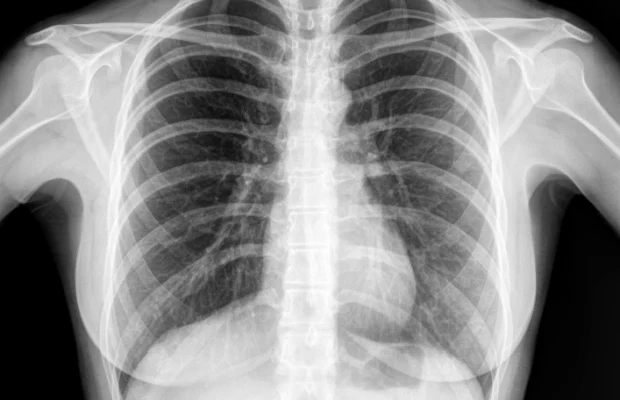
\includegraphics[width=0.85\linewidth]{Figures/xray.jpg}
    \\ \vspace{0.5em}
    {\tiny \color{gray!50} 2D Projection View}
\end{columns}
\end{frame}

%%%%%%%%%%%%%%%%%%%%%%%%%%%%%%%%%%%%%%%%%%%%%%%%


% \begin{frame}{Medical Imaging: X-Ray}
% \small

% \begin{columns}[c,onlytextwidth] % center vertically

%     \column{0.58\linewidth}

%     \textbf{Imaging Mechanism}\\
%     High-energy electromagnetic radiation is transmitted through the body.

%     \vspace{0.7em}

%     \textbf{Key ideas}
%     \begin{itemize}
%         \item \textbf{Attenuation:} Dense structures (bone) absorb more $\rightarrow$ appear bright.
%         \item \textbf{Projection:} 2D shadow image of 3D anatomy.
%     \end{itemize}

%     \vspace{0.5em}

%     \textbf{Clinical Applciations}
%     \begin{itemize}
%         \item Bone fractures
%         \item Dental imaging
%         \item Chest screening (e.g., pneumonia)
%     \end{itemize}

%     \column{0.42\linewidth}

%     \centering
%     \vspace{0.5em}
%     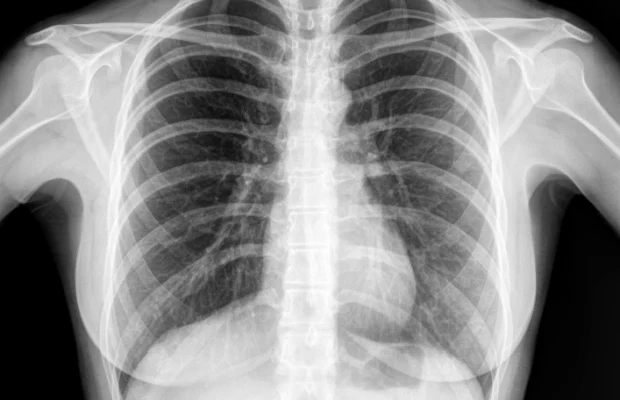
\includegraphics[width=0.9\linewidth]{Figures/xray.jpg}

% \end{columns}

% \end{frame}


\begin{frame}{Medical Imaging: Computed Tomography (CT)}
\small
\begin{columns}[c,onlytextwidth]

    \column{0.55\linewidth}
    
    % Physics Block
    \uncover<2->{\begin{tcolorbox}[standard jigsaw, 
        opacityback=0.08, opacityframe=0.3, 
        colback=teal, colframe=gray!70!black,
        colupper=white,
        title=\textbf{\color{teal!30}Imaging Mechanism},
        arc=3pt]
        Rotating X-ray source + detectors reconstruct cross-sectional slices.
    \end{tcolorbox}}

    \vspace{0.3em}

    % Key Concepts Block
    \uncover<3->{\begin{tcolorbox}[standard jigsaw, 
        opacityback=0.03, opacityframe=0.1, 
        colback=white, colframe=white, 
        colupper=white,
        title=\textbf{\color{teal!30}Technical Features}, 
        arc=3pt]
        \begin{itemize}
            \item {Hounsfield Units (HU)}. 
            \item {Tomographic Reconstruction}. 
        \end{itemize}
    \end{tcolorbox}}
    %%%%%%%%%%%%%%%%%%%%%%%%% NOTES %%%%%%%%%%%%%%%%%
    % \item[-] \textbf{Hounsfield Units (HU):} Quantitative radiodensity scale for tissue characterization.
    % \item[-] \textbf{Tomographic Reconstruction:} Multiple projections $\Rightarrow$ cross-sectional slices and 3D volume.
    %%%%%%%%%%%%%%%%%%%%%%%%% NOTES %%%%%%%%%%%%%%%%%   
    \vspace{0.3em}

    % Best For Block
    \uncover<4->{\begin{tcolorbox}[standard jigsaw, 
        opacityback=0.1, opacityframe=0.3, 
        colback=gray, colframe= teal!60!black, 
        colupper=white,
        title=\textbf{\color{teal!30}Clinical Applications}, 
        arc=3pt]
        Complex fractures, trauma assessment, internal bleeding, tumor detection and staging.
    \end{tcolorbox}}
    

    \column{0.45\linewidth}
    \centering
    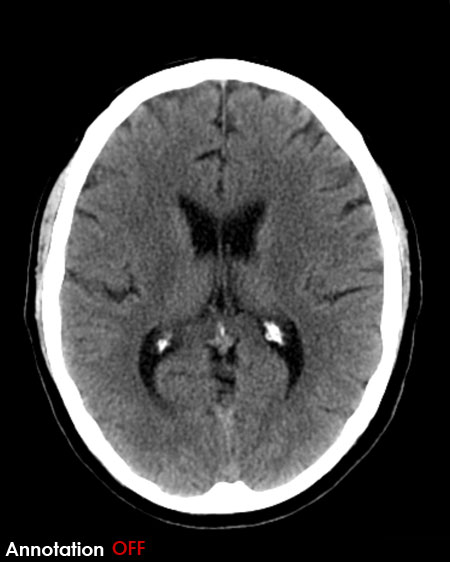
\includegraphics[width=0.85\linewidth]{Figures/ct.jpg}
    \\ \vspace{0.5em}
    {\tiny \color{gray!50} Cross-sectional \& 3D View}

\end{columns}
\end{frame}

% -----------------------------
% \begin{frame}{Medical Imaging: Computed Tomography (CT)}
% \small
% \begin{columns}[T,onlytextwidth]

%     \column{0.56\linewidth}
%     \textbf{Mechanism:} Rotating X-ray source + detectors reconstruct cross-sectional slices.

%     \vspace{0.4em}
%     \textbf{Key ideas}
%     \begin{itemize}
%         \item \textbf{Hounsfield Units (HU):} Quantitative radiodensity scale.
%         \item \textbf{3D reconstruction:} Stack slices to visualize anatomy volumetrically.
%     \end{itemize}

%     \vspace{0.4em}
%     \textbf{Clinical Applciations}
%     \begin{itemize}
%         \item Complex fractures / trauma
%         \item Internal bleeding
%         \item Tumor detection + staging
%     \end{itemize}

%     \column{0.44\linewidth}
%     \centering
%     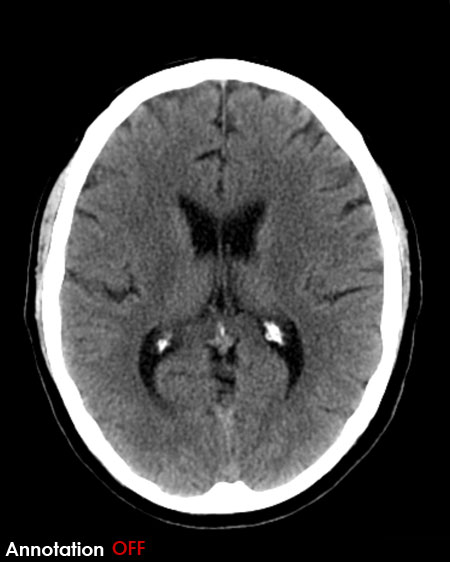
\includegraphics[width=\linewidth]{Figures/ct.jpg}

% \end{columns}
% \end{frame}

\begin{frame}{Medical Imaging: MRI}
\small
\begin{columns}[c,onlytextwidth]

    \column{0.55\linewidth}
    
    % Physics Block
    \uncover<2->{\begin{tcolorbox}[standard jigsaw, 
        opacityback=0.08, opacityframe=0.3, 
        colback=teal, colframe=gray!70!black,
        colupper=white,
        title=\textbf{\color{teal!30}Imaging Mechanism},
        arc=3pt]
        Strong magnetic fields + RF pulses excite hydrogen nuclei; signals are reconstructed into images.
    \end{tcolorbox}}

    \vspace{0.3em}

    % Key Concepts Block
    \uncover<3->{\begin{tcolorbox}[standard jigsaw, 
        opacityback=0.03, opacityframe=0.1, 
        colback=white, colframe=white, 
        colupper=white,
        title=\textbf{\color{teal!30}Technical Features}, 
        arc=3pt]
        \begin{itemize}
            \item {No Ionizing Radiation}.
            \item {Soft-Tissue Contrast}.
            \item {T1 vs T2}.
        \end{itemize}
    \end{tcolorbox}}
    %%%%%%%%%%%%%%%%%%%%%%%%% NOTES %%%%%%%%%%%%%%%%%
    % \item[-] \textbf{No Ionizing Radiation:} Safer for repeated imaging.
    % \item[-] \textbf{Soft-Tissue Contrast:} Excellent for brain, muscles, ligaments.
    % \item[-] \textbf{T1 vs T2:} Fat appears bright in T1; fluid appears bright in T2.
    %%%%%%%%%%%%%%%%%%%%%%%%% NOTES %%%%%%%%%%%%%%%%%   

    \vspace{0.3em}

    % Best For Block
    \uncover<4->{\begin{tcolorbox}[standard jigsaw, 
        opacityback=0.1, opacityframe=0.3, 
        colback=gray, colframe= teal!60!black, 
        colupper=white,
        title=\textbf{\color{teal!30}Clinical Applications}, 
        arc=3pt]
        Brain and spinal cord imaging, ligament and tendon injuries, pelvic and abdominal soft tissues.
    \end{tcolorbox}}

    \column{0.45\linewidth}
    \centering
    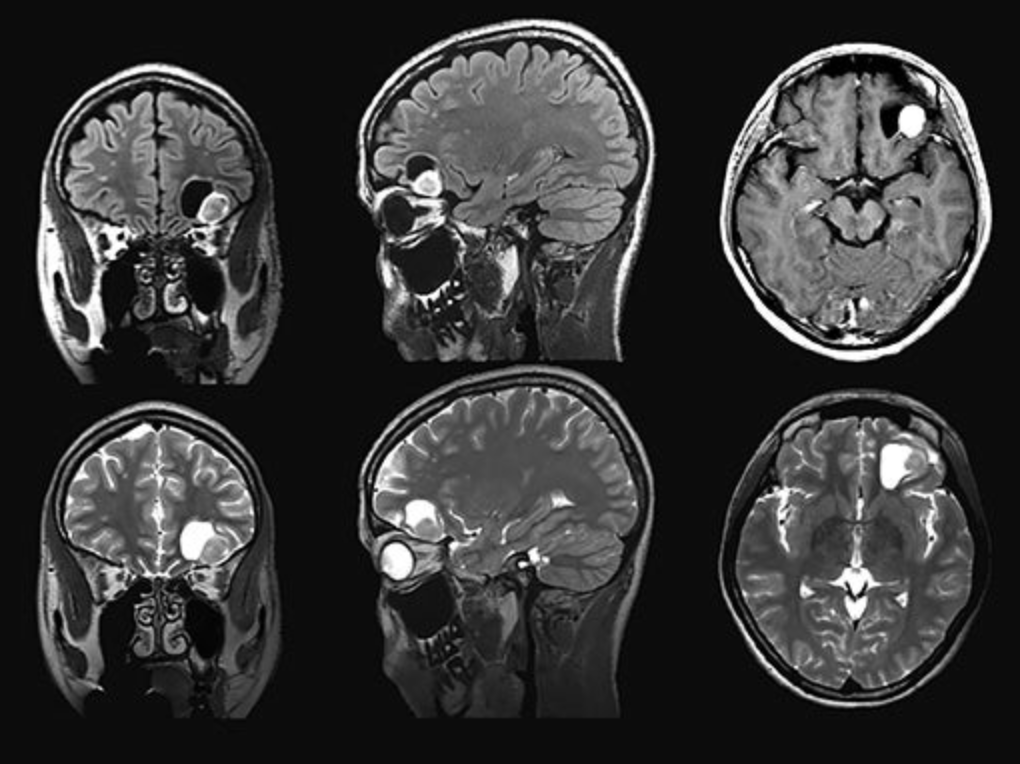
\includegraphics[width=0.85\linewidth, trim=1cm 0cm 0cm 0cm, clip]{Figures/mri.png}
    \\ \vspace{0.5em}
    {\tiny \color{gray!50} High Soft-Tissue Contrast}

\end{columns}
\end{frame}

% -----------------------------


% \begin{frame}{Medical Imaging: MRI}
% \small

% \begin{columns}[c,onlytextwidth]

%     \column{0.58\linewidth}

%     \textbf{Mechanism}\\
%     Strong magnetic fields + RF pulses excite hydrogen nuclei; signals are reconstructed into images.

%     \vspace{0.7em}

%     \textbf{Key ideas}
%     \begin{itemize}
%         \item \textbf{No ionizing radiation:} safer for repeated imaging.
%         \item \textbf{Soft-tissue contrast:} excellent for brain, muscles, ligaments.
%         \item \textbf{Common sequences:} T1 (fat bright) vs.\ T2 (fluid bright).
%     \end{itemize}

%     \vspace{0.5em}

%     \textbf{Clinical Applciations}
%     \begin{itemize}
%         \item Brain and spinal cord
%         \item Ligament / tendon injuries
%         \item Pelvic and abdominal soft tissues
%     \end{itemize}

%     \column{0.42\linewidth}

%     \centering
%     \vspace{0.5em}
%     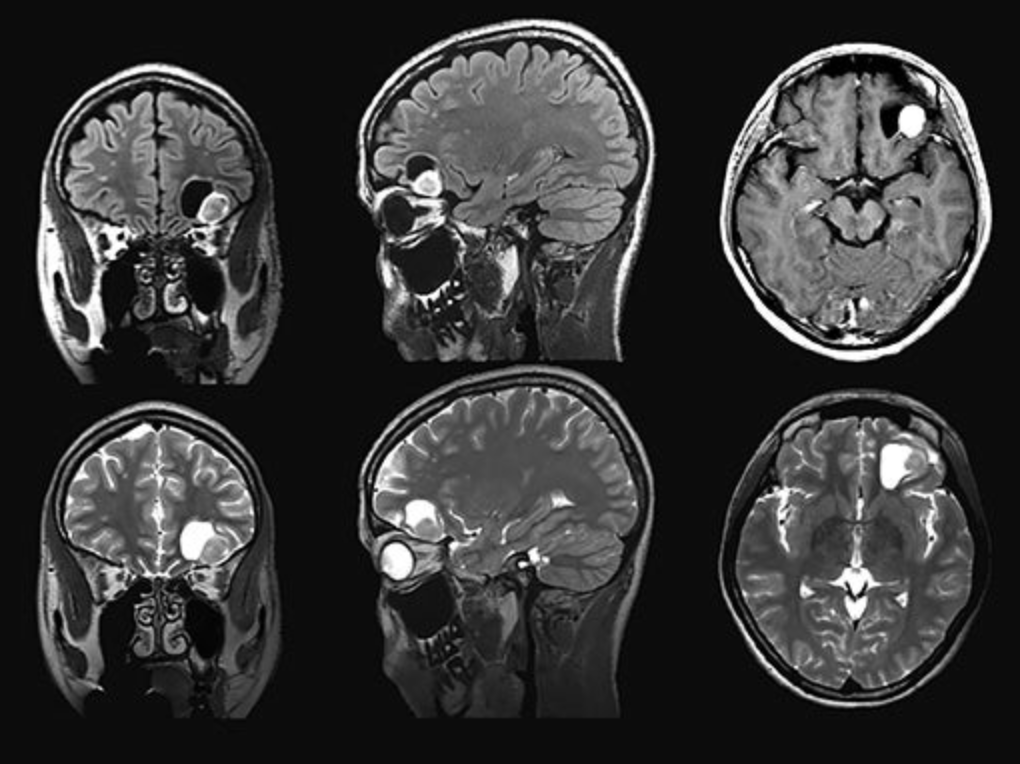
\includegraphics[width=0.9\linewidth, trim=1cm 0cm 0cm 0cm, clip]{Figures/mri.png}

% \end{columns}

% \end{frame}

%%%%%%%%%%%%%%%%%%%%%%%%%%%%%%%%%%%%%%%%%%%%%%%%

% -----------------------------
% \begin{frame}{}
% \vfill
% \centering
% \usebeamerfont{title}
% \huge What kind of analysis task would we want to\\[0.3em]
% do using these images?
% \vfill
% \end{frame}


\makepart{Analytical Task}

% -----------------------------
\begin{frame}{Common Tasks in Medical Image Analysis}
\small

% \begin{columns}[c,onlytextwidth]

%     \column{0.42\linewidth}
    \centering
    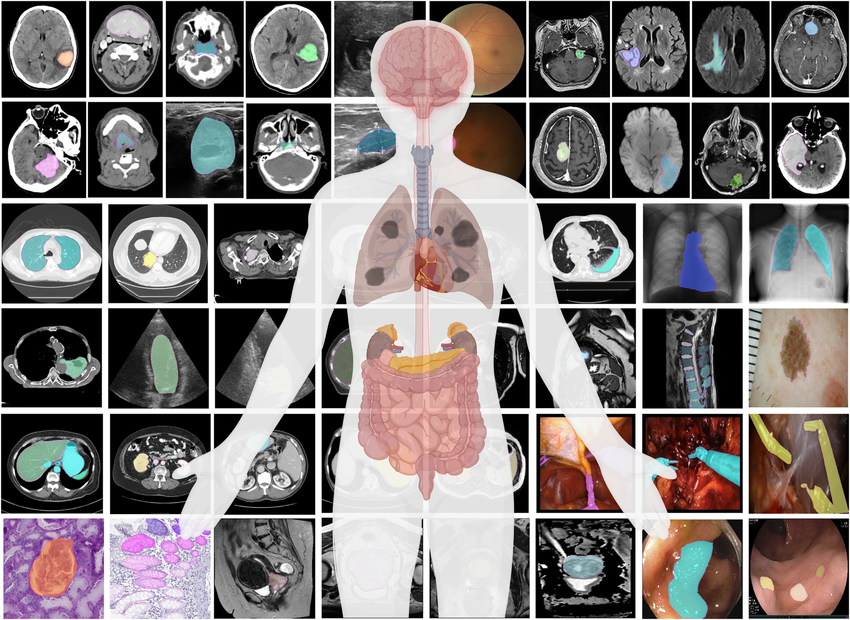
\includegraphics[width=0.9\linewidth]{Figures/MedSAM.png}

%     \column{0.58\linewidth}

%     \textbf{Typical tasks}
%     \vspace{0.4em}

%     \begin{itemize}\setlength\itemsep{0.35em}
%         \item \textbf{Image preprocessing}: super resolution, densification
%         \item \textbf{Registration}: align spatial coordinates across modalities (e.g.\ PET + MRI)
%         \item \textbf{Detection}: highlighting specific elements (anomaly/lesion)
%         \item \textbf{Segmentation}: delineation or volume extraction of target object (organ/lesion)
%         \item \textbf{Classification}: distinguish classes of objects (benign vs malignant lesion)
%         \item \textbf{Monitoring}: longitudinal measurement of lesion (\% of organ impacted)
%         \item \textbf{Prediction}: predicting outcome based on image (e.g.\ chemotherapy response)
%     \end{itemize}

% \end{columns}

\vfill
\begin{flushleft}
\tiny Source: \href{https://doi.org/10.1186/s13244-019-0832-5}{Lassau et al., Insights Imaging 2019}
\end{flushleft}

\end{frame}

%------------------------------
\begin{frame}{Common Tasks in Medical Image Analysis}
\centering

\begin{tikzpicture}[
    scale=0.44, transform shape, 
    font=\sffamily\color{white},
    phasebox/.style={
        rectangle, rounded corners=10pt, draw, thick,
        minimum width=7cm, 
        minimum height=5.8cm,
        align=center, 
        fill = black, %fill=black!85, 
        text width=7cm, 
        inner sep=3pt,
        text=white,
        font = \huge
    },
    nodenumber/.style={
        circle, draw, ultra thick, fill=black, text=white,
        minimum size=1.4cm, font=\huge\bfseries,
        inner sep=0pt, font = \huge
    },
    mainarrow/.style={
    -{Stealth[length=10pt, width=6pt]}, % larger, clearer arrowhead
    line width=2.2pt,                   % slightly thicker for emphasis
    line cap=round,
    line join=round,
    shorten >=0pt,
    shorten <=0pt
    },
    vertline/.style={
        -, 
        line width=1pt,   % THINNER VERTICAL LINE
        line cap=round,
        shorten >=0pt,
        shorten <=0pt
    },
    bgcolumn/.style={
        rounded corners=5pt,  % increase this for smoother corners
        minimum width=7.8cm, 
        minimum height=22cm, 
        inner sep=0pt,
        outer sep=0pt,
        anchor=center,
        fill opacity = 0.6
    }
]

% --- Image Helper Command ---
\newcommand{\boximage}[1]{%
    \begin{minipage}[c][4cm][c]{6cm}  % slightly larger than image
        \centering
        \includegraphics[width=5.5cm, height=4cm, keepaspectratio]{Figures/##1}
    \end{minipage}\\[0.3cm]
}

% --- Colors ---




% --- 1. COORDINATES ---
\coordinate (p1) at (0,0);
\coordinate (p2) at (7.8,0);
\coordinate (p3) at (15.6,0);
\coordinate (p4) at (23.4,0);

% --- 2. BACKGROUND LAYER ---
\begin{scope}[on background layer]
    \node[bgcolumn, fill=bgTeal] at (p1) {}; %\node[bgcolumn, fill=bgTeal] at (p1) {};
    \node[bgcolumn, fill=bgGreen] at (p2) {};
    \node[bgcolumn, fill=bgAmber] at (p3) {};
    \node[bgcolumn, fill=bgCoral] at (p4) {};
\end{scope}


% --- 3. PHASE BOXES ---
\node[phasebox, draw=accTeal, above=2.5cm of p1] (top1) {\boximage{superResolution} \textbf{\Huge Preprocessing:} super resolution}; % https://mriquestions.com/super-resolution.html
\node[phasebox, draw=accTeal, below=2.5cm of p1] (bot1) {\boximage{registered-final} \textbf{\Huge Registration:}\\align coordinates};  %https://3dqlab.stanford.edu/image-registration/

\node[phasebox, draw=accGreen, above=2.5cm of p2] (top2) {\boximage{object-detection-medical-imaging} \textbf{\Huge Detection:}\\highlight elements};%https://www.imaios.com/en/resources/blog/introduction-to-the-most-common-deep-learning-architectures-for-object-detection-in-medical-imaging
\node[phasebox, draw=accGreen, below=2.5cm of p2] (bot2) {\boximage{segmentation} \textbf{\Huge Segmentation:}\\volume delineation};   %https://www.nature.com/articles/s41467-024-44824-z/figures/2

\node[phasebox, draw=accAmber, below=2.5cm of p3] (bot3) {\boximage{classification} \textbf{\Huge Classification:}\\distinguish classes}; %https://www.sciencedirect.com/science/article/pii/S1877750324001170
\node[phasebox, draw=accAmber, above=2.5cm of p3] (top3) {\boximage{cell} \textbf{\Huge Classification:}\\identify cell types}; %https://pmc.ncbi.nlm.nih.gov/articles/PMC11810770/

\node[phasebox, draw=accCoral, above=2.5cm of p4] (top4) {\boximage{longitudinal} \textbf{\Huge Monitoring:}\\longitudinal study}; %https://journals.plos.org/plosone/article?id=10.1371/journal.pone.0049072
\node[phasebox, draw=accCoral, below=2.5cm of p4] (bot4) {\boximage{outcome} \textbf{\Huge Prediction:}\\outcome analysis}; %https://news.mit.edu/2019/ai-model-atlas-patient-brain-analysis-1126

% --- 4. TITLES ---
\node[above=9.5cm of p1, font=\huge\bfseries] {PREPARATION};
\node[above=9.5cm of p2, font=\huge\bfseries] {FEATURE};
\node[above=9.5cm of p3, font=\huge\bfseries] {OBJECT};
\node[above=9.5cm of p4, font=\huge\bfseries] {OUTCOME};

% --- 5. DRAWING LINES ---
\draw[vertline, accTeal] (top1) -- (bot1);
\draw[vertline, accGreen] (top2) -- (bot2);
\draw[vertline, accAmber] (top3) -- (bot3);
\draw[vertline, accCoral] (top4) -- (bot4);

\draw[mainarrow, accTeal] (-3.9,0) -- (p1);
\draw[mainarrow, accGreen] (p1) -- (p2);
\draw[mainarrow, accAmber] (p2) -- (p3);
\draw[mainarrow, accCoral] (p3) -- (p4);
\draw[mainarrow, accCoral] (p4) -- (27.3,0);

% --- 6. NUMBERED CIRCLES (LAST = ON TOP) ---
\node[nodenumber, draw=accTeal] at (p1) {1};
\node[nodenumber, draw=accGreen] at (p2) {2};
\node[nodenumber, draw=accAmber] at (p3) {3};
\node[nodenumber, draw=accCoral] at (p4) {4};

\end{tikzpicture}

\end{frame}
%------------------------------


\begin{frame}{Common Tasks in Medical Image Analysis}
\centering
\begin{tikzpicture}[
    scale=0.44, transform shape, 
    font=\sffamily\color{white},
    phasebox/.style={
        rectangle, rounded corners=10pt, draw, thick,
        minimum width=7cm, 
        minimum height=5.8cm,
        align=center, 
        fill = black, %fill=black!85, 
        text width=7cm, 
        inner sep=3pt,
        text=white,
        font = \huge
    },
    nodenumber/.style={
        circle, draw, ultra thick, fill=black, text=white,
        minimum size=1.4cm, font=\huge\bfseries,
        inner sep=0pt, font = \huge
    },
    mainarrow/.style={
    -{Stealth[length=10pt, width=6pt]}, % larger, clearer arrowhead
    line width=2.2pt,                   % slightly thicker for emphasis
    line cap=round,
    line join=round,
    shorten >=0pt,
    shorten <=0pt
    },
    vertline/.style={
        -, 
        line width=1pt,   % THINNER VERTICAL LINE
        line cap=round,
        shorten >=0pt,
        shorten <=0pt
    },
    bgcolumn/.style={
        rounded corners=5pt,  % increase this for smoother corners
        minimum width=7.8cm, 
        minimum height=22cm, 
        inner sep=0pt,
        outer sep=0pt,
        anchor=center,
        fill opacity = 0.6
    }
]

% --- Image Helper Command ---
\newcommand{\boximage}[1]{%
    \begin{minipage}[c][4cm][c]{6cm} 
        \centering
        \includegraphics[width=5.5cm, height=4cm, keepaspectratio]{Figures/##1}
    \end{minipage}\\[0.3cm]
}

% --- Colors ---
\definecolor{accTeal}{RGB}{77, 208, 225}
\definecolor{accGreen}{RGB}{129, 199, 132}
\definecolor{accAmber}{RGB}{255, 213, 79}
\definecolor{accCoral}{RGB}{255, 138, 101}

\definecolor{bgTeal}{RGB}{15, 30, 40}
\definecolor{bgGreen}{RGB}{15, 30, 20}
\definecolor{bgAmber}{RGB}{30, 25, 10}
\definecolor{bgCoral}{RGB}{35, 15, 15}

% --- 1. COORDINATES ---
\coordinate (p1) at (0,0);
\coordinate (p2) at (7.8,0);
\coordinate (p3) at (15.6,0);
\coordinate (p4) at (23.4,0);

% --- 2. BACKGROUND LAYER ---
\begin{scope}[on background layer]
    \node[bgcolumn, fill=bgTeal] at (p1) {};
    \node[bgcolumn, fill=bgGreen] at (p2) {};
    \node[bgcolumn, fill=bgAmber] at (p3) {};
    \node[bgcolumn, fill=bgCoral] at (p4) {};
\end{scope}

% --- 3. PHASE BOXES ---
\node[phasebox, draw=accTeal, above=2.5cm of p1] (top1) {\boximage{superResolution} \textbf{\Huge Preprocessing:} super resolution};
\node[phasebox, draw=accTeal, below=2.5cm of p1] (bot1) {\boximage{registered-final} \textbf{\Huge Registration:}\\align coordinates}; 

\node[phasebox, draw=accGreen, above=2.5cm of p2] (top2) {\boximage{object-detection-medical-imaging} \textbf{\Huge Detection:}\\highlight elements};
\node[phasebox, draw=accGreen, below=2.5cm of p2] (bot2) {\boximage{segmentation} \textbf{\Huge Segmentation:}\\volume delineation};    

\node[phasebox, draw=accAmber, below=2.5cm of p3] (bot3) {\boximage{classification} \textbf{\Huge Classification:}\\distinguish classes};
\node[phasebox, draw=accAmber, above=2.5cm of p3] (top3) {\boximage{cell} \textbf{\Huge Classification:}\\identify cell types};

\node[phasebox, draw=accCoral, above=2.5cm of p4] (top4) {\boximage{longitudinal} \textbf{\Huge Monitoring:}\\longitudinal study};
\node[phasebox, draw=accCoral, below=2.5cm of p4] (bot4) {\boximage{outcome} \textbf{\Huge Prediction:}\\outcome analysis};

% --- 4. TITLES ---
\node[above=9.5cm of p1, font=\huge\bfseries] {PREPARATION};
\node[above=9.5cm of p2, font=\huge\bfseries] {FEATURE};
\node[above=9.5cm of p3, font=\huge\bfseries] {OBJECT};
\node[above=9.5cm of p4, font=\huge\bfseries] {OUTCOME};

% --- 5. DRAWING LINES ---
\draw[vertline, accTeal] (top1) -- (bot1);
\draw[vertline, accGreen] (top2) -- (bot2);
\draw[vertline, accAmber] (top3) -- (bot3);
\draw[vertline, accCoral] (top4) -- (bot4);

\draw[mainarrow, accTeal] (-3.9,0) -- (p1);
\draw[mainarrow, accGreen] (p1) -- (p2);
\draw[mainarrow, accAmber] (p2) -- (p3);
\draw[mainarrow, accCoral] (p3) -- (p4);
\draw[mainarrow, accCoral] (p4) -- (27.3,0);

% --- 6. NUMBERED CIRCLES ---
\node[nodenumber, draw=accTeal] at (p1) {1};
\node[nodenumber, draw=accGreen] at (p2) {2};
\node[nodenumber, draw=accAmber] at (p3) {3};
\node[nodenumber, draw=accCoral] at (p4) {4};

% --- 7. THE ANIMATION OVERLAY (SHROUD) ---
% This creates the black transparency over blocks. 
% On slide 1, blocks 2,3,4 are covered. On slide 2, blocks 1,3,4 are covered, etc.
\begin{scope}
    % Block 1 Shroud (Visible on slides 2, 3, 4)
    \fill<2-4>[black, opacity=0.7, rounded corners=5pt] ($(p1)+(-3.9,-11)$) rectangle ($(p1)+(3.9,11)$);
    
    % Block 2 Shroud (Visible on slides 1, 3, 4)
    \fill<1,3-4>[black, opacity=0.7, rounded corners=5pt] ($(p2)+(-3.9,-11)$) rectangle ($(p2)+(3.9,11)$);
    
    % Block 3 Shroud (Visible on slides 1, 2, 4)
    \fill<1-2,4>[black, opacity=0.7, rounded corners=5pt] ($(p3)+(-3.9,-11)$) rectangle ($(p3)+(3.9,11)$);
    
    % Block 4 Shroud (Visible on slides 1, 2, 3)
    \fill<1-3>[black, opacity=0.7, rounded corners=5pt] ($(p4)+(-3.9,-11)$) rectangle ($(p4)+(3.9,11)$);
\end{scope}

\end{tikzpicture}

\end{frame}




%%%%%%%%%%%%%%%%%%%%%%%%%%%%%%%%%%%%%%%%%%%%%%%%
\begin{frame}{Medical Image Data is Intrinsically challenging }
\small
\begin{columns}[T,onlytextwidth]

    % -------- LEFT COLUMN --------
    \column{0.45\linewidth}

    % (1,1) Small Data Paradox
    \uncover<1->{\begin{tcolorbox}[standard jigsaw, 
        opacityback=0.1, opacityframe=0.3, 
        colback=gray, colframe=teal!60!black, 
        colupper=white,
        title=\textbf{\color{teal!30}Small Data Paradox},
        arc=3pt]
        \vspace{1em}
        \alert<1>{Modalities}:\,\,\,High-res 3D volumes but few patient samples. \\ [1em]
        \alert<1>{Long-tail}:\,\,\,common diseases dominate; rare cases are hidden. \\ [2em]

        \hspace{2em}\begin{tikzpicture}[scale=0.55]
            \draw[->, thick, white!70] (0,0) -- (6,0);
            \draw[->, thick, white!70] (0,0) -- (0,4);
            
            \draw[ultra thick, coral, smooth] 
                (0.2,3.8) .. controls (0.5,0.5) and (2,0.2) .. (5.5,0.1);
            
            \fill[coral, opacity=0.3] 
                (0.2,3.8) .. controls (0.5,0.5) and (2,0.2) .. (5.5,0.1)
                -- (5.5,0) -- (0.2,0) -- cycle;

            \node[coral!80, font=\tiny] at (1.2,3.2) {Common};
            \node[white!80, font=\tiny] at (4.2,0.6) {Rare};
        \end{tikzpicture}


        {\scriptsize \color{gray!50} Imbalance: common vs.\ rare diseases} \vspace{0.5em}
    \end{tcolorbox}
    }

    % -------- RIGHT COLUMN --------
    \column{0.5\linewidth}

    % (2,1) Technical Variability  <-- moved here
    \uncover<2->{\begin{tcolorbox}[standard jigsaw, 
        opacityback=0.08, opacityframe=0.3, 
        colback=coral, colframe=gray!70!black,
        colupper=white,
        title=\textbf{\color{teal!30}Technical Variability}, 
        arc=3pt]
        \vspace{1em}
         \alert<2>{Non-standard}:\,\,\,vendors (Siemens vs.\ GE), protocols differ. \\ [1em]
         \alert<2>{Subjective labels}:\,\,\,inter observer variability. \\
    \end{tcolorbox}}

    \vspace{0.4em}

    % (2,2) Privacy Constraints
    \uncover<3->{\begin{tcolorbox}[standard jigsaw, 
        opacityback=0.08, opacityframe=0.3, 
        colback=teal, colframe=gray!70!black,
        colupper=white,
        title=\textbf{\color{teal!30}Privacy Constraints},
        arc=3pt]
        \vspace{1em}
        \alert<3>{De-identification risk} (e.g., facial reconstruction). \\[1em]
        Siloed data due to HIPAA / GDPR constraints.
    \end{tcolorbox}}

\end{columns}
\end{frame}

% -----------------------------
% \begin{frame}{Medical image data is intrinsically challenging}
% \begin{itemize}\setlength\itemsep{0.4em}
%     \item Lots of modalities with very large image size (but small datasets)
%     \item Non-standardised acquisition (varied devices, set-ups etc)
%     \item Disease patterns in images are very long-tailed
%     %\item Labels are sparse and noisy
%     \item Samples are heterogeneous and imbalanced
%     \item Subjectivity in ground-truth
%     \item Privacy and de-identification e.g., facial scans
% \end{itemize}
% \end{frame}
\begin{frame}{Patient can have many imaging modalities}
\small
\begin{columns}[T,onlytextwidth]

    \column{0.60\linewidth}
    65 year old female presents to \textit{\underline{Emergency}} with sudden facial drooping and arm weakness:

    \vspace{1em}
    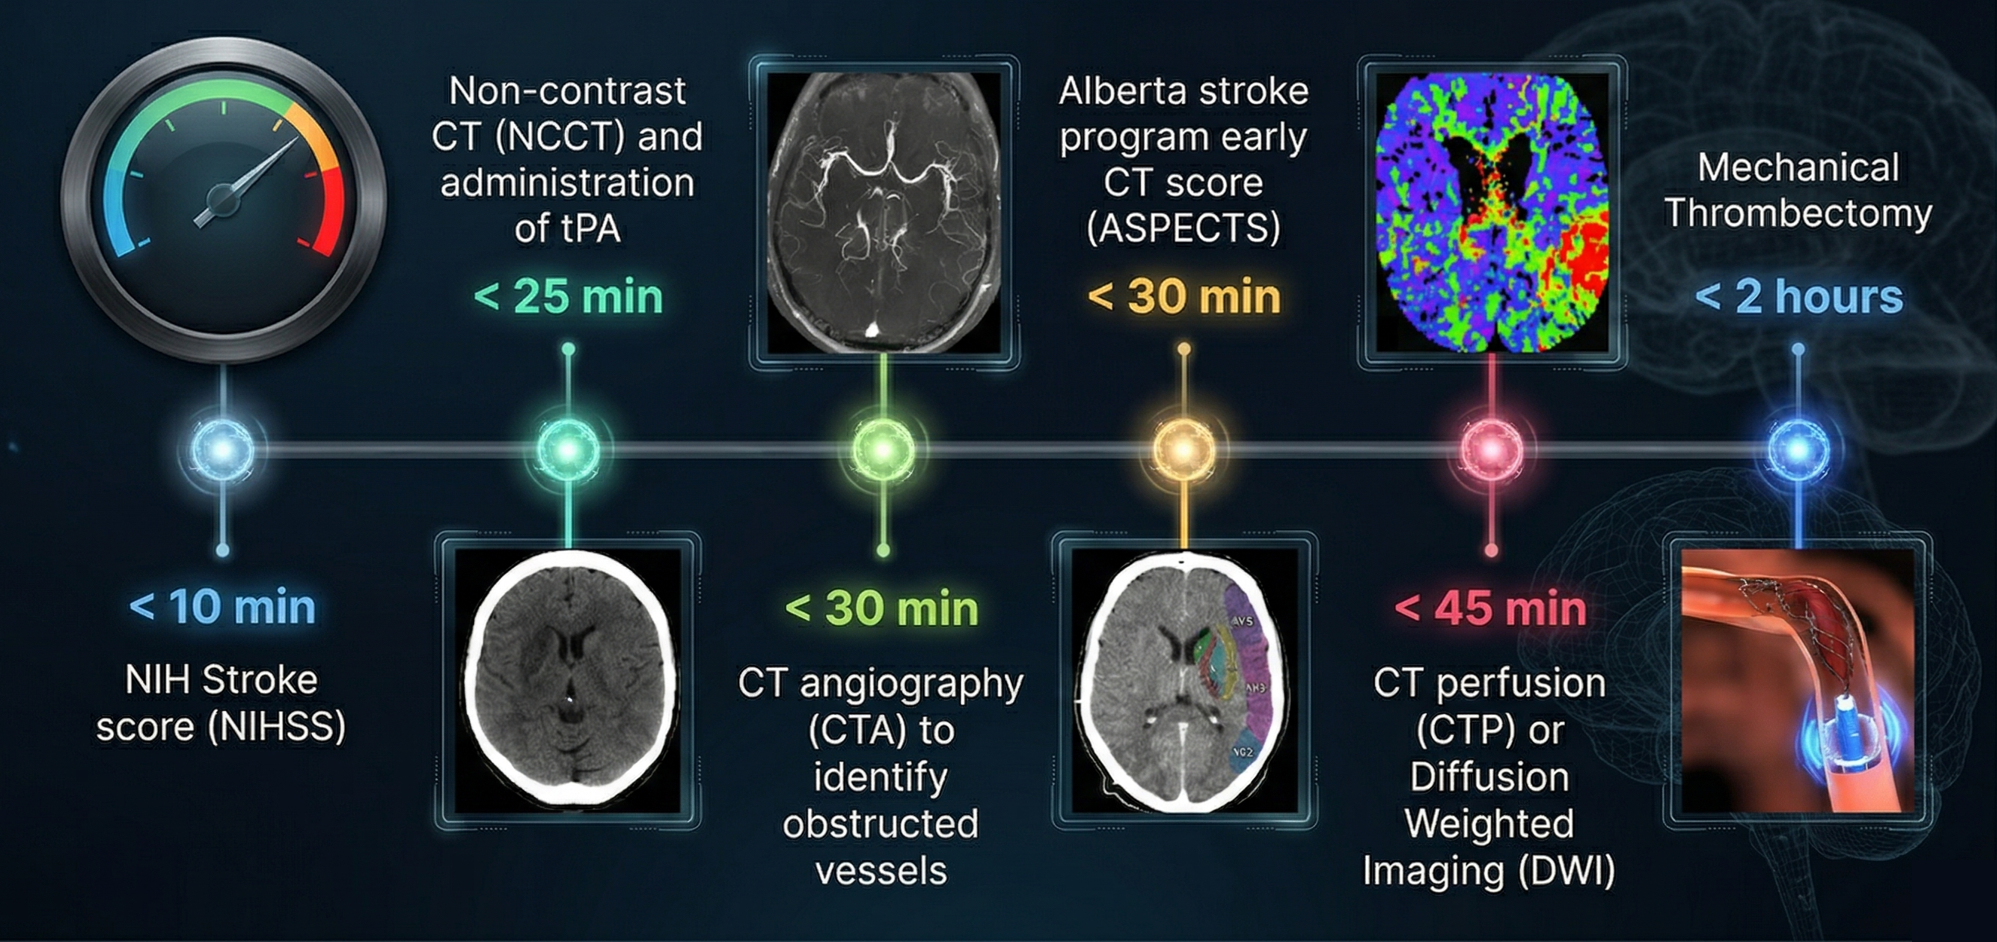
\includegraphics[width=1.5\linewidth]{Figures/protocol.PNG}

\end{columns}
\end{frame}


%%%%%%%%%%%%%%%%%%%%%%%%%%%%%%%%%%%%%%%%%%%%%%%%


% -----------------------------
% \begin{frame}{Patient can have many imaging modalities}
% \small
% \begin{columns}[T,onlytextwidth]

%     \column{0.60\linewidth}
%     65 year old female presents to \textit{\underline{Emergency}} with sudden facial drooping and arm weakness:

%     \vspace{0.3em}
%     % \begin{enumerate}
%     %     \item \textit{\underline{Emergency}} performs \textbf{CT} (non-contrast) to exclude haemorrhagic stroke
%     %     \item \textit{\underline{Radiology}} performs \textbf{CT Angiography} to identify large vessel occlusion
%     %     \item \textit{\underline{Neurology}} reviews deficit; \textbf{MRI/DWI} confirms ischaemic penumbra
%     %     \item \textit{\underline{Interventional Radiology}} performs \textbf{DSA}-guided mechanical thrombectomy
%     %     \item \textit{\underline{Radiology}} performs follow-up \textbf{MRI} to assess reperfusion and infarct extent
%     %     \item \textit{\underline{Cardiology}} performs \textbf{echocardiography} to detect cardioembolic source (e.g.\ AF)
%     %     \item \textit{\underline{Radiology}} performs \textbf{carotid ultrasound} to evaluate atherosclerotic stenosis
%     %     \item Patient returns to \textit{\underline{Neurology}} clinic; \textbf{MRI} repeated to monitor recovery
%     %     \item \textit{\underline{Nuclear Medicine}} performs \textbf{SPECT-CT} for cerebral perfusion mapping
%     % \end{enumerate}

%     \vspace{0.4em}
%     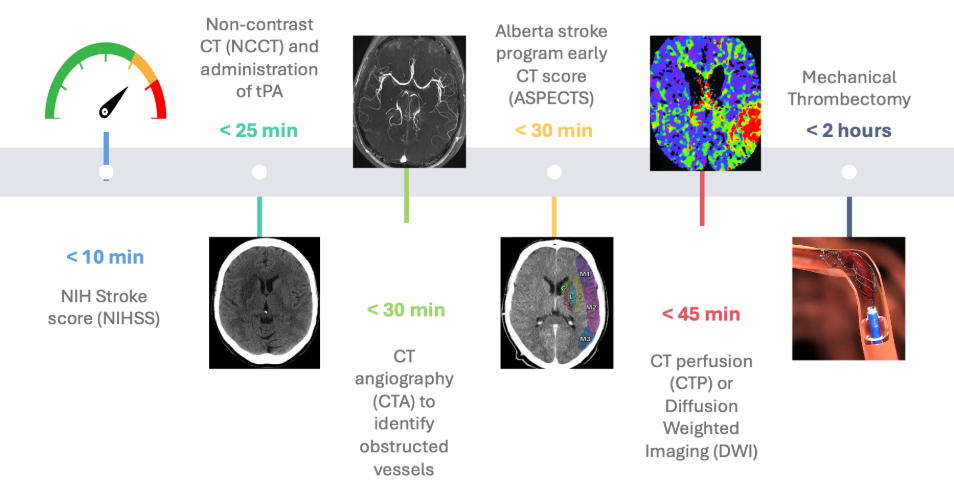
\includegraphics[width=1.5\linewidth]{Figures/stroke_protocal.png}

% \end{columns}
% \end{frame}

% % -----------------------------
% \begin{frame}[t]{Early Acute Ischemic Stroke: Care Management Flow}
% \vspace{0.4em}
% \begin{center}
% \resizebox{\linewidth}{!}{%
% \begin{tikzpicture}[
%   font=\sffamily\scriptsize,
%   pre/.style={rounded corners=3pt, draw=cyan!60, fill=cyan!12!black,
%               text=white, align=center, minimum width=2.8cm, inner sep=3pt, line width=0.8pt},
%   ed/.style={rounded corners=3pt, draw=orange!70, fill=orange!10!black,
%              text=white, align=center, minimum width=2.8cm, inner sep=3pt, line width=0.8pt},
%   act/.style={rounded corners=3pt, draw=green!60, fill=green!12!black,
%               text=white, align=center, minimum width=3.0cm, inner sep=3pt, line width=0.8pt},
%   lbl/.style={text=yellow!90, font=\sffamily\tiny\bfseries},
%   arr/.style={->, >=stealth, white, line width=0.9pt},
%   cross/.style={->, >=stealth, yellow!80, line width=0.8pt, dashed},
% ]

% %% === ROW 1: horizontal prehospital + early ED ===
% \node[pre] (recog) at (0, 0)
%   {\textbf{RECOGNITION}\\(by bystander)};
% \node[pre] (assess) at (3.5, 0)
%   {\textbf{ASSESS FOR STROKE (I)}\\F.A.S.T.\ $\cdot$ CPSS $\cdot$ LAPSS};
% \node[pre] (fmc) at (7.4, 0)
%   {\textbf{FIRST MEDICAL CONTACT (II)}\\ABCs $\cdot$ O$_2{>}94\%$\\IV access $\cdot$ Notify hospital};
% \node[ed]  (nihss) at (11.0, 0)
%   {\textbf{NIHSS (III)}\\Emergency Dept};
% \node[ed]  (diag) at (14.8, 0)
%   {\textbf{IMMEDIATE DIAGNOSTICS (IV)}\\NCCT $\cdot$ Blood glucose $\cdot$ CBC\\PT/INR $\cdot$ ECG $\cdot$ O$_2$ sat};

% %% === ROW 2: parallel evaluation ===
% \node[ed] (eval_iv) at (12.2, -2.8)
%   {\textbf{EVALUATE FOR}\\IV ALTEPLASE (V)\\$\leq$ 4.5 h from onset};
% \node[ed] (eval_mt) at (17.4, -2.8)
%   {\textbf{EVALUATE FOR}\\MECH.\ THROMBECTOMY (VI)\\$<$ 24 h (select patients)};

% %% === ROW 3: administer ===
% \node[act] (adm_iv) at (12.2, -5.4)
%   {\textbf{ADMINISTER IV ALTEPLASE (VII)}\\0.9 mg/kg (max 90 mg) IV 60 min\\Admit ICU/stroke unit $\geq$ 24 h};
% \node[act] (adm_mt) at (17.4, -5.4)
%   {\textbf{ADMINISTER MT (VIII)}\\Stent retriever\\BP $\leq$ 180/105 mmHg};

% %% === ARROWS ===
% \draw[arr] (recog)  -- (assess);
% \draw[arr] (assess) -- node[above, lbl]{POSITIVE} (fmc);
% \draw[arr] (fmc)    -- (nihss);
% \draw[arr] (nihss)  -- (diag);
% \draw[arr] (diag.south)  -- ++(0,-0.45) -| (eval_iv.north);
% \draw[arr] (diag.south)  -- ++(0,-0.45) -| (eval_mt.north);
% \draw[arr] (eval_iv) -- node[left,  lbl]{QUALIFIES} (adm_iv);
% \draw[arr] (eval_mt) -- node[right, lbl]{QUALIFIES} (adm_mt);
% \draw[cross] (adm_iv.east) -- node[above, lbl]{QUALIFIES FOR MT} (adm_mt.west);

% %% === LABELS ===
% \node[lbl] at ($(eval_iv.north east)!0.5!(eval_mt.north west)$)
%   {SIMULTANEOUS};

% % Vertical phase-separator between fmc and nihss
% \draw[white!30, dashed, thin]
%   ($(fmc.north east)+(0.3, 0.3)$) -- ($(fmc.south east)+(0.3,-0.3)$);

% % Phase labels (above row 1)
% \node[text=cyan!75, font=\sffamily\tiny\bfseries]
%   at ($(recog.north)!0.5!(fmc.north)+(0,0.35)$) {OUT OF HOSPITAL};
% \node[text=orange!80, font=\sffamily\tiny\bfseries]
%   at ($(nihss.north)!0.5!(diag.north)+(0,0.35)$) {EMERGENCY DEPT};

% \end{tikzpicture}%
% }
% \end{center}
% \end{frame}


%%%%%%%%%%%%%%%%%%%%%%%%%%%%%%%%%%%%%%%%%%%%%%%%
\makepart{History of Computer Vision}


%%%%%%%%%%%%%%%%%%%%%%%%%%%%%%%%%%%%%%%%%%%%%%%%

\begin{frame}{{Traditional Computer Vision}}

\begin{columns}[T,onlytextwidth]

% -------- LEFT COLUMN --------
\column{0.55\linewidth}


% \begin{tcolorbox}[standard jigsaw, 
%         opacityback=0.08, opacityframe=0.3, 
%         colback=teal, colframe=gray!70!black,
%         colupper=white,
%         title=\textbf{\color{teal!30}Core Techniques},
%         arc=3pt]
     \textbf{\Large \color{teal!30}Core Techniques} \\ [1em]

    \begin{itemize}
        \item  \alert<1>{{Thresholding}} \\
    {\small Pixels $\geq$ a value $\rightarrow$ set to maximum} \\[1em] 

     \item  \alert<2>{{Edge Detection}} \\
    {\small Detect changes in brightness}\\[1em]

    \item   \alert<3>{{Segmentation}} \\
    {\small Group regions enclosed by edges} \\[1em]

     \item  \alert<4>{{Curve Detection}} \\
    {\small Link adjacent edges into shapes} \\[1em]

     \item  \alert<5>{{Optical Flow}} \\
    {\small Estimate motion between frames}
    \end{itemize}
        
% \end{tcolorbox}



% -------- RIGHT COLUMN --------
\column{0.45\linewidth}

\vspace{5em}
    \centering
    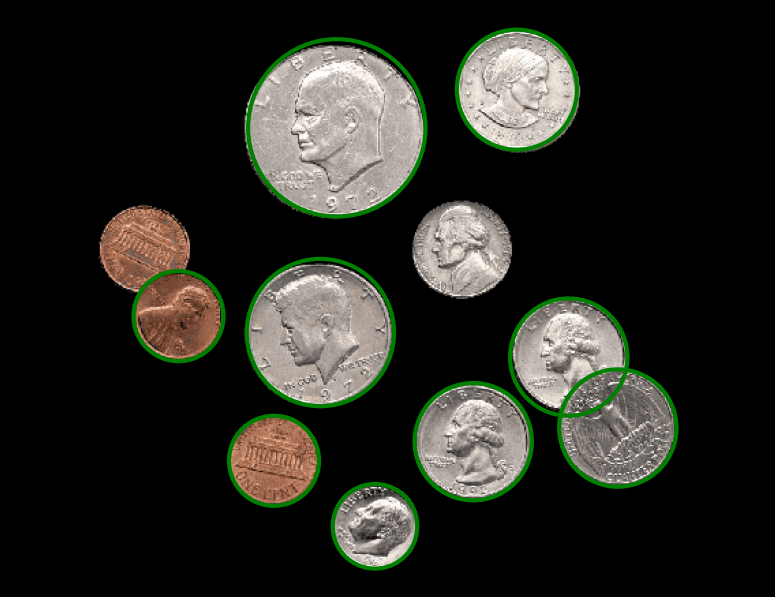
\includegraphics[width=0.9\linewidth]{Figures/coin.png}
    \vspace{2em}
    {\tiny \textcolor{gray}{Source: pyimagesearch.com}}


\end{columns}

\uncover<6->{
\vspace{1em}
\begin{center}
    {\alert{Classical pipeline}: Pixels $\rightarrow$ Edges $\rightarrow$ Shapes $\rightarrow$ Motion}
\end{center}
}

\end{frame}


% -----------------------------
% \begin{frame}{Traditional Computer Vision}
% \begin{columns}[T,onlytextwidth]

%     \column{0.55\linewidth}
%     \begin{itemize}\setlength\itemsep{0.35em}
%         \item \textbf{Thresholding}: pixels $\geq$ certain value set to max
%         \item \textbf{Edge detection}: changes in brightness
%         \item \textbf{Segmenting}: grouping thresholded areas enclosed by edges
%         \item \textbf{Curve detection}: edges adjacent to one another
%         \item \textbf{Optical flow}: detection of movement
%     \end{itemize}

%     \vspace{1.2em}
%     \centering
%     % % ---- Curve detection illustration ----
%     % \begin{tikzpicture}[scale=0.85]
%     %     % Template corner (L-shape)
%     %     \draw[green!60!white, line width=1.2pt] (0,0.35) -- (0,0) -- (0.35,0);
%     %     \draw[green!60!white, line width=1.2pt] (0.07,0.35) -- (0.07,0.07) -- (0.35,0.07);
%     %     % Arrow
%     %     \draw[->, green!50!white, line width=1.5pt] (0.55,0.17) -- (1.05,0.17);
%     %     % Curve
%     %     \draw[white!80, line width=1.2pt]
%     %         (1.3,-0.15) .. controls (1.6,0.9) and (2.5,0.9) .. (3.3,0.25);
%     %     % Green squares at curve points
%     %     \foreach \px/\py in {1.42/0.18, 1.65/0.62, 2.05/0.80, 2.55/0.72, 3.05/0.43} {
%     %         \fill[green!65!white] (\px-0.09,\py-0.09) rectangle (\px+0.09,\py+0.09);
%     %     }
%     % \end{tikzpicture}

%     \column{0.45\linewidth}
%     \centering
%     % ---- Coins image ----
%     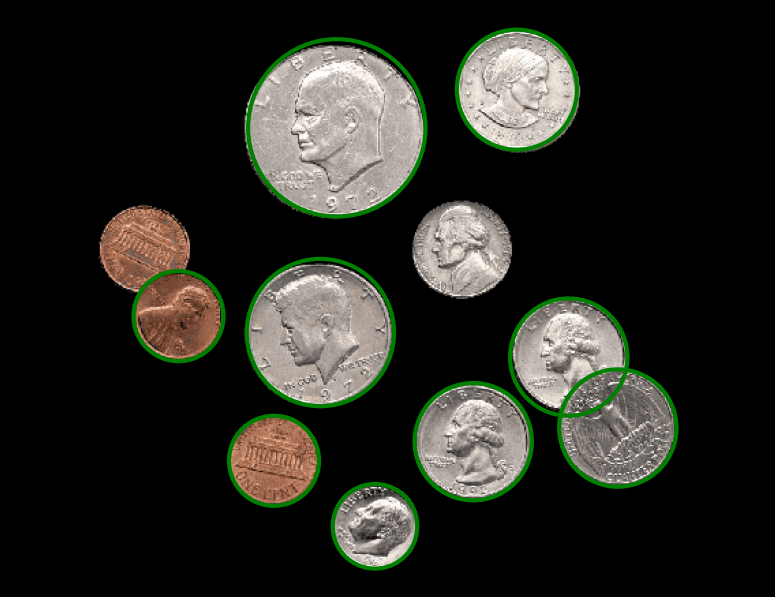
\includegraphics[width=0.92\linewidth]{Figures/coin.png}

%     \vspace{0.2em}
%     \begin{flushright}
%         \tiny \href{https://pyimagesearch.com/2021/04/28/opencv-thresholding-cv2-threshold/}{pyimagesearch.com}
%     \end{flushright}

% \end{columns}
% \end{frame}



%%%%%%%%%%%%%%%%%%%%%%%%%%%%%%%%%%%%%%%%%%%%%%%%
% \begin{frame}{Feature Engineering: Sobel Filters}

% \vfill
% \centering
% 
\includegraphics[width = 0.8\textwidth]{edgeDetection.png}
    

%     \begin{flushleft}
%         \tiny Source: \href{https://www.geeksforgeeks.org/computer-vision/what-is-edge-detection-in-image-processing/}{Geeks}
%     \end{flushleft}
    
% \end{frame}

%%%%%%%%%%%%%%%%%%%%%%%%%%%%%%%%%%%%%%%%%%%%%%%%
\begin{frame}{Feature Engineering: Sobel Filters}

\small

\begin{columns}[T,onlytextwidth] % use only the text area (respects margins)

% -------- LEFT COLUMN --------
\column{0.5\linewidth}

\alert<1>{\textbf{Edge}}: {a location where image intensity changes abruptly.}

\vspace{2em}

\alert<2>{\textbf{Intuition}}
\begin{itemize}
    \item {Flat region $\rightarrow$ small intensity change}
    \item {Object boundary $\rightarrow$ sharp intensity change}
\end{itemize}

\vspace{0.4em}

{
    Treat the \alert<2>{image as a function} $f(x,y)$:
    \[
    {\nabla f} =
    \begin{bmatrix}
    \frac{\partial f}{\partial x}\\[2pt]
    \frac{\partial f}{\partial y}
    \end{bmatrix}
    \]
}

{
    Edge strength (gradient magnitude):
    \[
    \alert<3>{\|\nabla f\|} =
    \sqrt{
    \left(\frac{\partial f}{\partial x}\right)^2 +
    \left(\frac{\partial f}{\partial y}\right)^2
    }
    \]
}

% -------- RIGHT COLUMN --------
\column{0.45\linewidth}

\alert<3>{\textbf{Goal}}: {find pixels where the gradient magnitude is large.}

\vspace{2em}


    \alert<4>{\textbf{Practical Significance}}
    \begin{itemize}
    \item Extract object boundaries
    \item Reduce data complexity
    \item Basis for segmentation / recognition
    \end{itemize}
    
\vspace{1em}

\alert<5>{\textbf{Steps}}
\begin{itemize}
    \item {Compute derivatives}
    \item {Compute gradient magnitude}
    \item {Threshold / keep large values}
    \uncover<6>{\item[$\Rightarrow$] \alert{ SOBEL filter}}
\end{itemize}



\end{columns}

\end{frame}
%%%%%%%%%%%%%%%%%%%%%%%%%%%%%%%%%%%%%%%%%%%%%%%%




%%%%%%%%%%%%%%%%%%%%%%%%%%%%%%%%%%%%%%%%%%%%%%%%

\begin{frame}{Sobel Filter: Vertical Edge Detection}
\centering

% (Best practice: move these \definecolor lines to the preamble,
%  but keeping them here works if you only use them on this slide.)
\definecolor{kRed}{RGB}{255,200,200}
\definecolor{kGreen}{RGB}{200,255,200}
\definecolor{pxDark}{RGB}{60,60,60}
\definecolor{pxLight}{RGB}{240,240,240}
\definecolor{textGreen}{rgb}{0, 0.4, 0}

\begin{columns}[c,onlytextwidth]

    % ---------------- Image Patch ----------------
    \column{0.29\linewidth}
    \centering
    \textbf{\footnotesize Image Patch ($I$)}\\[0.35em]
    \resizebox{\linewidth}{!}{%
        \begin{tikzpicture}
            \foreach \y in {0,1,2} {
                \draw[fill=pxDark] (0,\y) rectangle (1,\y+1) node[pos=.5, white] {\tiny 10};
                \draw[fill=pxDark] (1,\y) rectangle (2,\y+1) node[pos=.5, white] {\tiny 10};
                \draw[fill=pxLight] (2,\y) rectangle (3,\y+1) node[pos=.5, black] {\tiny 200};
            }
            \node at (1.5,-0.4) {\tiny Dark $\to$ Bright};
        \end{tikzpicture}%
    }

    % ---------------- Convolution symbol ----------------
    \column{0.05\linewidth}
    \centering \Large $\ast$

    % ---------------- Sobel Kernel ----------------
    \column{0.29\linewidth}
    \centering
    \textbf{\footnotesize Sobel Kernel ($G_x$)}\\[0.35em]
    \resizebox{\linewidth}{!}{%
        \begin{tikzpicture}
        \foreach \y/\w in {0/1, 1/2, 2/1} {
            \draw[fill=kRed] (0,\y) rectangle (1,\y+1)
                node[pos=.5, text=black] {\footnotesize -\w};
    
            \draw[fill=gray!10] (1,\y) rectangle (2,\y+1)
                node[pos=.5, text=black] {\footnotesize 0};
    
            \draw[fill=kGreen] (2,\y) rectangle (3,\y+1)
                node[pos=.5, text=black] {\footnotesize \w};
        }
    
        \node[text=black] at (1.5,-0.4) {\tiny Edge Weighting};
    \end{tikzpicture}
    }

    % ---------------- Equals symbol ----------------
    \column{0.05\linewidth}
    \centering \Large $=$

    % ---------------- Response ----------------
    \column{0.32\linewidth}
    \centering
    \textbf{\footnotesize Response}\\[0.35em]
    \resizebox{0.75\linewidth}{!}{%
        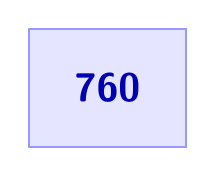
\begin{tikzpicture}[xshift = -3em] 
            \draw[fill=blue!10, draw=blue!40, thick]
                (0,0.75) rectangle (2,2.25)
                node[pos=.5, blue!70!black] {\Large \textbf{760}};
        \end{tikzpicture}%
    }

\end{columns}

\vspace{1em}

%%%%%%%%%%%%%%%%%%%%%%%%%%%%%%%
% \definecolor{accent}{RGB}{0,200,220}

% \setbeamercolor{frametitle}{fg=accent}
% \setbeamercolor{item}{fg=accent}
% \setbeamercolor{structure}{fg=accent}
% \setbeamercolor{normal text}{fg=white}
%%%%%%%%%%%%%%%%%%%%%%%%%%%%%%%

\pause
% Highlighted Calculation
\setbeamercolor{block body}{bg=gray!5,fg=black}
\begin{beamercolorbox}[wd=\linewidth, sep=6pt, center, rounded=true]{block body}
    \small
    Sum $= \textcolor{red!80!black}{(-1 \cdot 10)} + (0 \cdot 10) + \textcolor{textGreen}{(1 \cdot 200)} + \dots = \mathbf{760}$
\end{beamercolorbox}

% \begin{center}
% \begin{tikzpicture}
% \node[
%     fill=white,
%     fill opacity=0.2,
%     text opacity=1,
%     rounded corners,
%     inner sep=6pt,
%     text width=\linewidth,
%     align=center
% ] {
%     \small
%     Sum $= \textcolor{red!80!black}{(-1 \cdot 10)} + (0 \cdot 10) + \textcolor{textGreen}{(1 \cdot 200)} + \dots = \mathbf{760}$
% };
% \end{tikzpicture}
% \end{center}

\pause

\vspace{1.5em}

\begin{quote}\small
The \textbf{\textcolor{red!80!black}{negative weights}} suppress dark pixels, while
\textbf{\textcolor{textGreen}{positive weights}} amplify bright pixels.
A high response (760) indicates a strong \textbf{vertical edge}.
\end{quote}

\end{frame}



%%%%%%%%%%%%%%%%%%%%%%%%%%%%%%%%%%%%%%%%%%%%%%%%

\begin{frame}{Sobel Filter with Convolution}

\centering
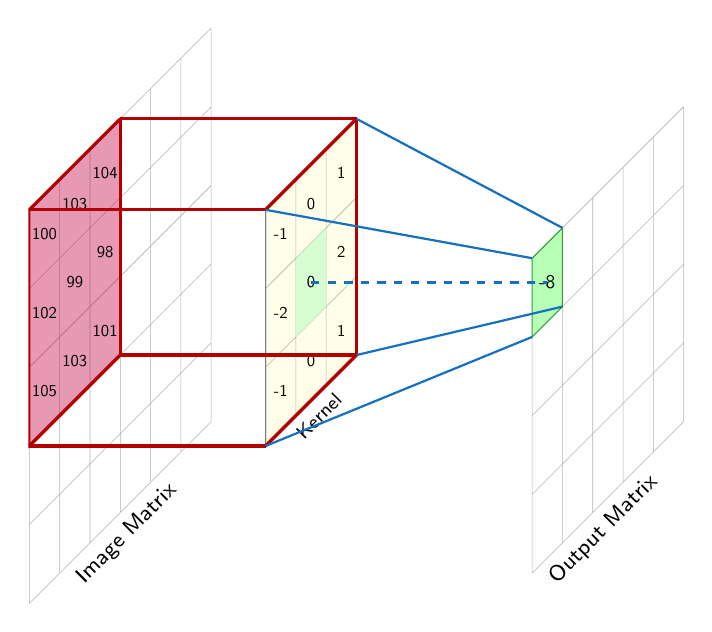
\begin{tikzpicture}[
    scale=1,
    grid line/.style={gray!60, very thin},
    matrix label/.style={font=\sffamily\bfseries},
    plane label/.style={matrix label, rotate=45, anchor=north west}
]

\tikzset{val/.style={scale=0.6, inner sep=0pt}}

% --- 1. Image Matrix ---
\begin{scope}[canvas is yz plane at x=0]
    \draw[grid line] (0,0) grid (5,6);

    \node[plane label, font=\footnotesize] at (0,5) {Image Matrix};

    % MOVE UP by 1: (2,2)-(5,5) -> (2,3)-(5,6)
    \fill[purple, opacity=0.4] (2,3) rectangle (5,6);
    \draw[red!70!black, thick] (2,3) rectangle (5,6);

    % Values shifted up by 1
    \foreach \c/\r/\val in {
        2/5/105, 3/5/102, 4/5/100,
        2/4/103, 3/4/99,  4/4/103,
        2/3/101, 3/3/98,  4/3/104
    }{
        \node[val] at (\c+0.5,\r+0.5) {\val};
    }
\end{scope}

% --- 2. Kernel Matrix ---
\begin{scope}[canvas is yz plane at x=3]

    % MOVE UP by 1: (2,2)-(5,5) -> (2,3)-(5,6)
    \fill[yellow!10, opacity=0.9, draw=black] (2,3) rectangle (5,6);
    \draw[grid line] (2,3) grid (5,6);

    \node[plane label, font=\scriptsize] at (2,5.5) {Kernel};

    % Kernel values shifted up
    \foreach \c/\r/\val in {
        0/2/-1,  1/2/-2, 2/2/-1,
        0/1/0,   1/1/0,  2/1/0,
        0/0/1,   1/0/2,  2/0/1
    }{
        \node[val, text = black] at (2+\c+0.5, 3+\r+0.5) {\val};
    }

    % Highlight center shifted up: (3,3)-(4,4) -> (3,4)-(4,5)
    \fill[green!20, opacity=0.8] (3,4) rectangle (4,5);
    \node[val, text = black] at (3.5,4.5) {0};
\end{scope}

% --- 3. Output Matrix ---
\begin{scope}[canvas is yz plane at x=6]
    \draw[grid line] (0,0) grid (4,5);

    \node[plane label, font=\footnotesize] at (0,5) {Output Matrix};

    % MOVE UP by 1: (3,3)-(4,4) -> (3,4)-(4,5)
    \fill[green!40, opacity=0.7, draw=green!50!black] (3,4) rectangle (4,5);
    \node[scale=0.7, text = black] at (3.5,4.5) {-8};
\end{scope}

% --- 4. Projection Lines (z +1) ---

\coordinate (iTL) at (0,5,3);
\coordinate (iTR) at (0,5,6);
\coordinate (iBL) at (0,2,3);
\coordinate (iBR) at (0,2,6);

\coordinate (kTL) at (3,5,3);
\coordinate (kTR) at (3,5,6);
\coordinate (kBL) at (3,2,3);
\coordinate (kBR) at (3,2,6);

\coordinate (oTL) at (6,4,4);
\coordinate (oTR) at (6,4,5);
\coordinate (oBL) at (6,3,4);
\coordinate (oBR) at (6,3,5);

\coordinate (kC) at (3,3.5,4.5);
\coordinate (oC) at (6,3.5,4.5);

% Red prism
\begin{scope}[red!70!black, very thick]
    \draw (iTL) -- (kTL);
    \draw (iTR) -- (kTR);
    \draw (iBL) -- (kBL);
    \draw (iBR) -- (kBR);

    \draw (iTL) -- (iTR);
    \draw (kTL) -- (kTR);

    \draw (iBL) -- (iBR);
    \draw (kBL) -- (kBR);

    \draw (iTL) -- (iBL);
    \draw (kTL) -- (kBL);
\end{scope}

% Blue projection
\begin{scope}[cyan!50!blue, thick]
    \draw (kTR) -- (oTR);
    \draw (kBR) -- (oBR);
    \draw (kTL) -- (oTL);
    \draw (kBL) -- (oBL);

    \draw[dashed] (kC) -- (oC);
\end{scope}

\end{tikzpicture}

\end{frame}


%%%%%%%%%%%%%%%%%%%%%%%%%%%%%%%%%%%%%%%%%%%%%%%%


\begin{frame}{Sobel Filter with Convolution (Slide Right + 1)}

\centering
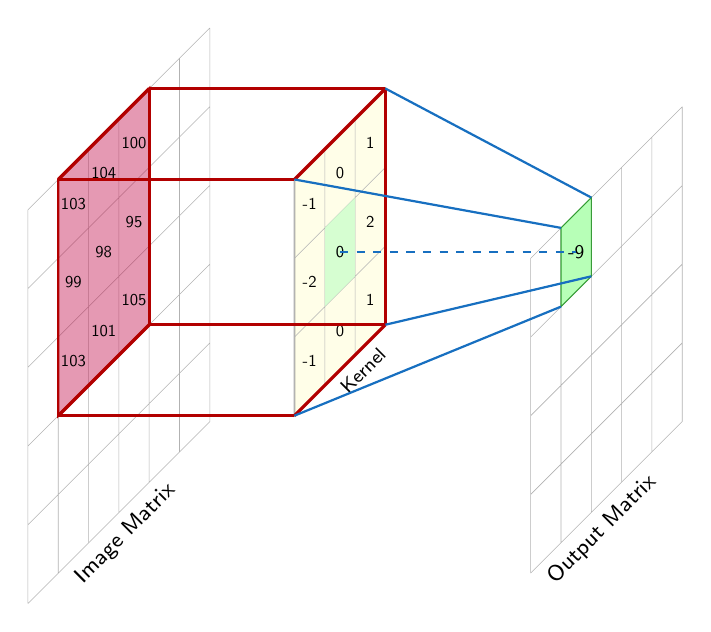
\begin{tikzpicture}[
    scale=1,
    grid line/.style={gray!60, very thin},
    matrix label/.style={font=\sffamily\bfseries},
    plane label/.style={matrix label, rotate=45, anchor=north west}
]

\tikzset{val/.style={scale=0.6, inner sep=0pt}}

% --- 1. Image Matrix ---
\begin{scope}[canvas is yz plane at x=0]
    \draw[grid line] (0,0) grid (5,6);

    \node[plane label, font=\footnotesize] at (0,5) {Image Matrix};

    % SHIFTED DOWN: was (2,3)-(5,6), now (2,2)-(5,5)
    \fill[purple, opacity=0.4] (2,2) rectangle (5,5);
    \draw[red!70!black, thick] (2,2) rectangle (5,5);

    % Values moved down by one row
    \foreach \c/\r/\val in {
        2/4/103, 3/4/99, 4/4/103,
        2/3/101, 3/3/98,  4/3/104,
        2/2/105, 3/2/95,  4/2/100
    }{
        \node[val] at (\c+0.5,\r+0.5) {\val};
    }
\end{scope}

% --- 2. Kernel Matrix ---
\begin{scope}[canvas is yz plane at x=3]
    % SHIFTED DOWN: was (2,3)-(5,6), now (2,2)-(5,5)
    \fill[yellow!10, opacity=0.9, draw=black] (2,2) rectangle (5,5);
    \draw[grid line] (2,2) grid (5,5);

    \node[plane label, font=\scriptsize] at (2,4) {Kernel};

    % Kernel values moved down
    \foreach \c/\r/\val in {
        0/2/-1,  1/2/-2, 2/2/-1,
        0/1/0, 1/1/0,  2/1/0,
        0/0/1,  1/0/2, 2/0/1
    }{
        \node[val, text = black] at (2+\c+0.5, 2+\r+0.5) {\val};
    }

    % Highlight center weight (shifted)
    \fill[green!20, opacity=0.8] (3,3) rectangle (4,4);
    \node[val, text = black] at (3.5,3.5) {0};
\end{scope}

% --- 3. Output Matrix ---
\begin{scope}[canvas is yz plane at x=6]
    \draw[grid line] (0,0) grid (4,5);

    \node[plane label, font=\footnotesize] at (0,5) {Output Matrix};

    % Output cell stays the same visually
    \fill[green!40, opacity=0.7, draw=green!50!black] (3,3) rectangle (4,4);
    \node[scale=0.7, text = black] at (3.5,3.5) {-9};
\end{scope}

% --- 4. Projection Lines (shifted down) ---
\coordinate (iTL) at (0,5,2);
\coordinate (iTR) at (0,5,5);
\coordinate (iBL) at (0,2,2);
\coordinate (iBR) at (0,2,5);

\coordinate (kTL) at (3,5,2);
\coordinate (kTR) at (3,5,5);
\coordinate (kBL) at (3,2,2);
\coordinate (kBR) at (3,2,5);

\coordinate (oTL) at (6,4,3);
\coordinate (oTR) at (6,4,4);
\coordinate (oBL) at (6,3,3);
\coordinate (oBR) at (6,3,4);


\coordinate (kC) at (3,3.5,3.5);
\coordinate (oC) at (6,3.5,3.5);

% Red prism (image -> kernel)
\begin{scope}[red!70!black, very thick]
    \draw (iTL) -- (kTL);
    \draw (iTR) -- (kTR);
    \draw (iBL) -- (kBL);
    \draw (iBR) -- (kBR);

    \draw (iTL) -- (iTR);
    \draw (kTL) -- (kTR);

    \draw (iBL) -- (iBR);
    \draw (kBL) -- (kBR);

    \draw (iTL) -- (iBL);
    \draw (kTL) -- (kBL);
\end{scope}

% Blue projection (kernel -> output)
\begin{scope}[cyan!50!blue, thick]
    \draw (kTR) -- (oTR);
    \draw (kBR) -- (oBR);
    \draw (kTL) -- (oTL);
    \draw (kBL) -- (oBL);

    \draw[dashed] (kC) -- (oC);
\end{scope}

\end{tikzpicture}

\end{frame}



%%%%%%%%%%%%%%%%%%%%%%%%%%%%%%%%%%%%%%%%%%%%%%%%







\begin{frame}{Feature Engineering: Template Matching}
\vfill

\centering
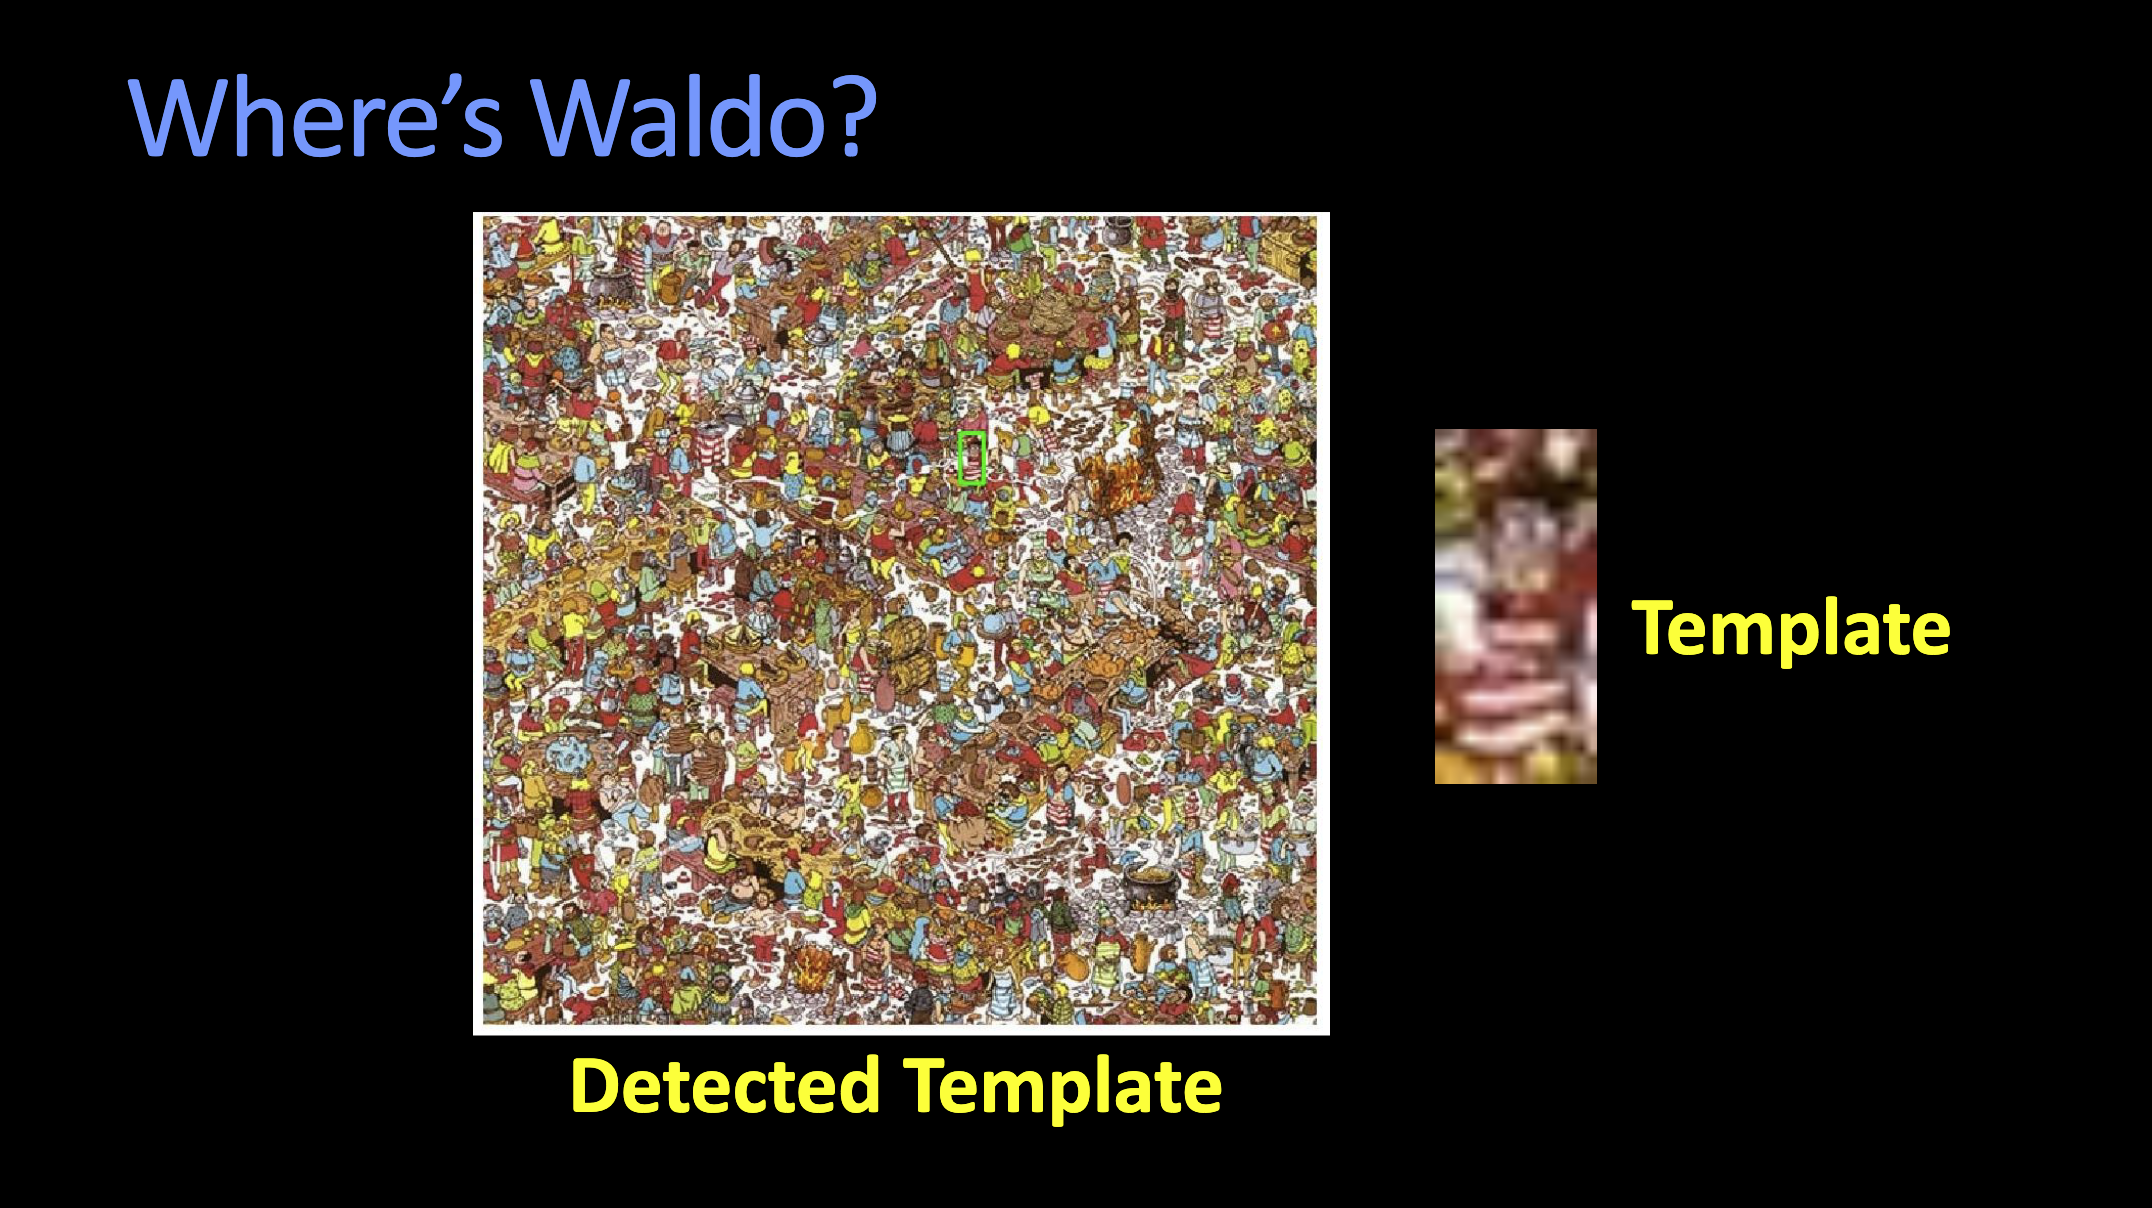
\includegraphics[width = 0.8\textwidth]{Figures/template-match.png}
    




    \begin{flushleft}
        \tiny Source: \href{https://omscs.gatech.edu/cs-6476-computer-vision}{GaTech computer Vision}
    \end{flushleft}
    
\end{frame}


%%%%%%%%%%%%%%%%%%%%%%%%%%%%%%%%%%%%%%%
%%%%%%%%%%%%%%%%%%%%%%%%%%%%%%%%%%%%%%%
\begin{frame}{Feature Engineering: Template Matching}

\centering
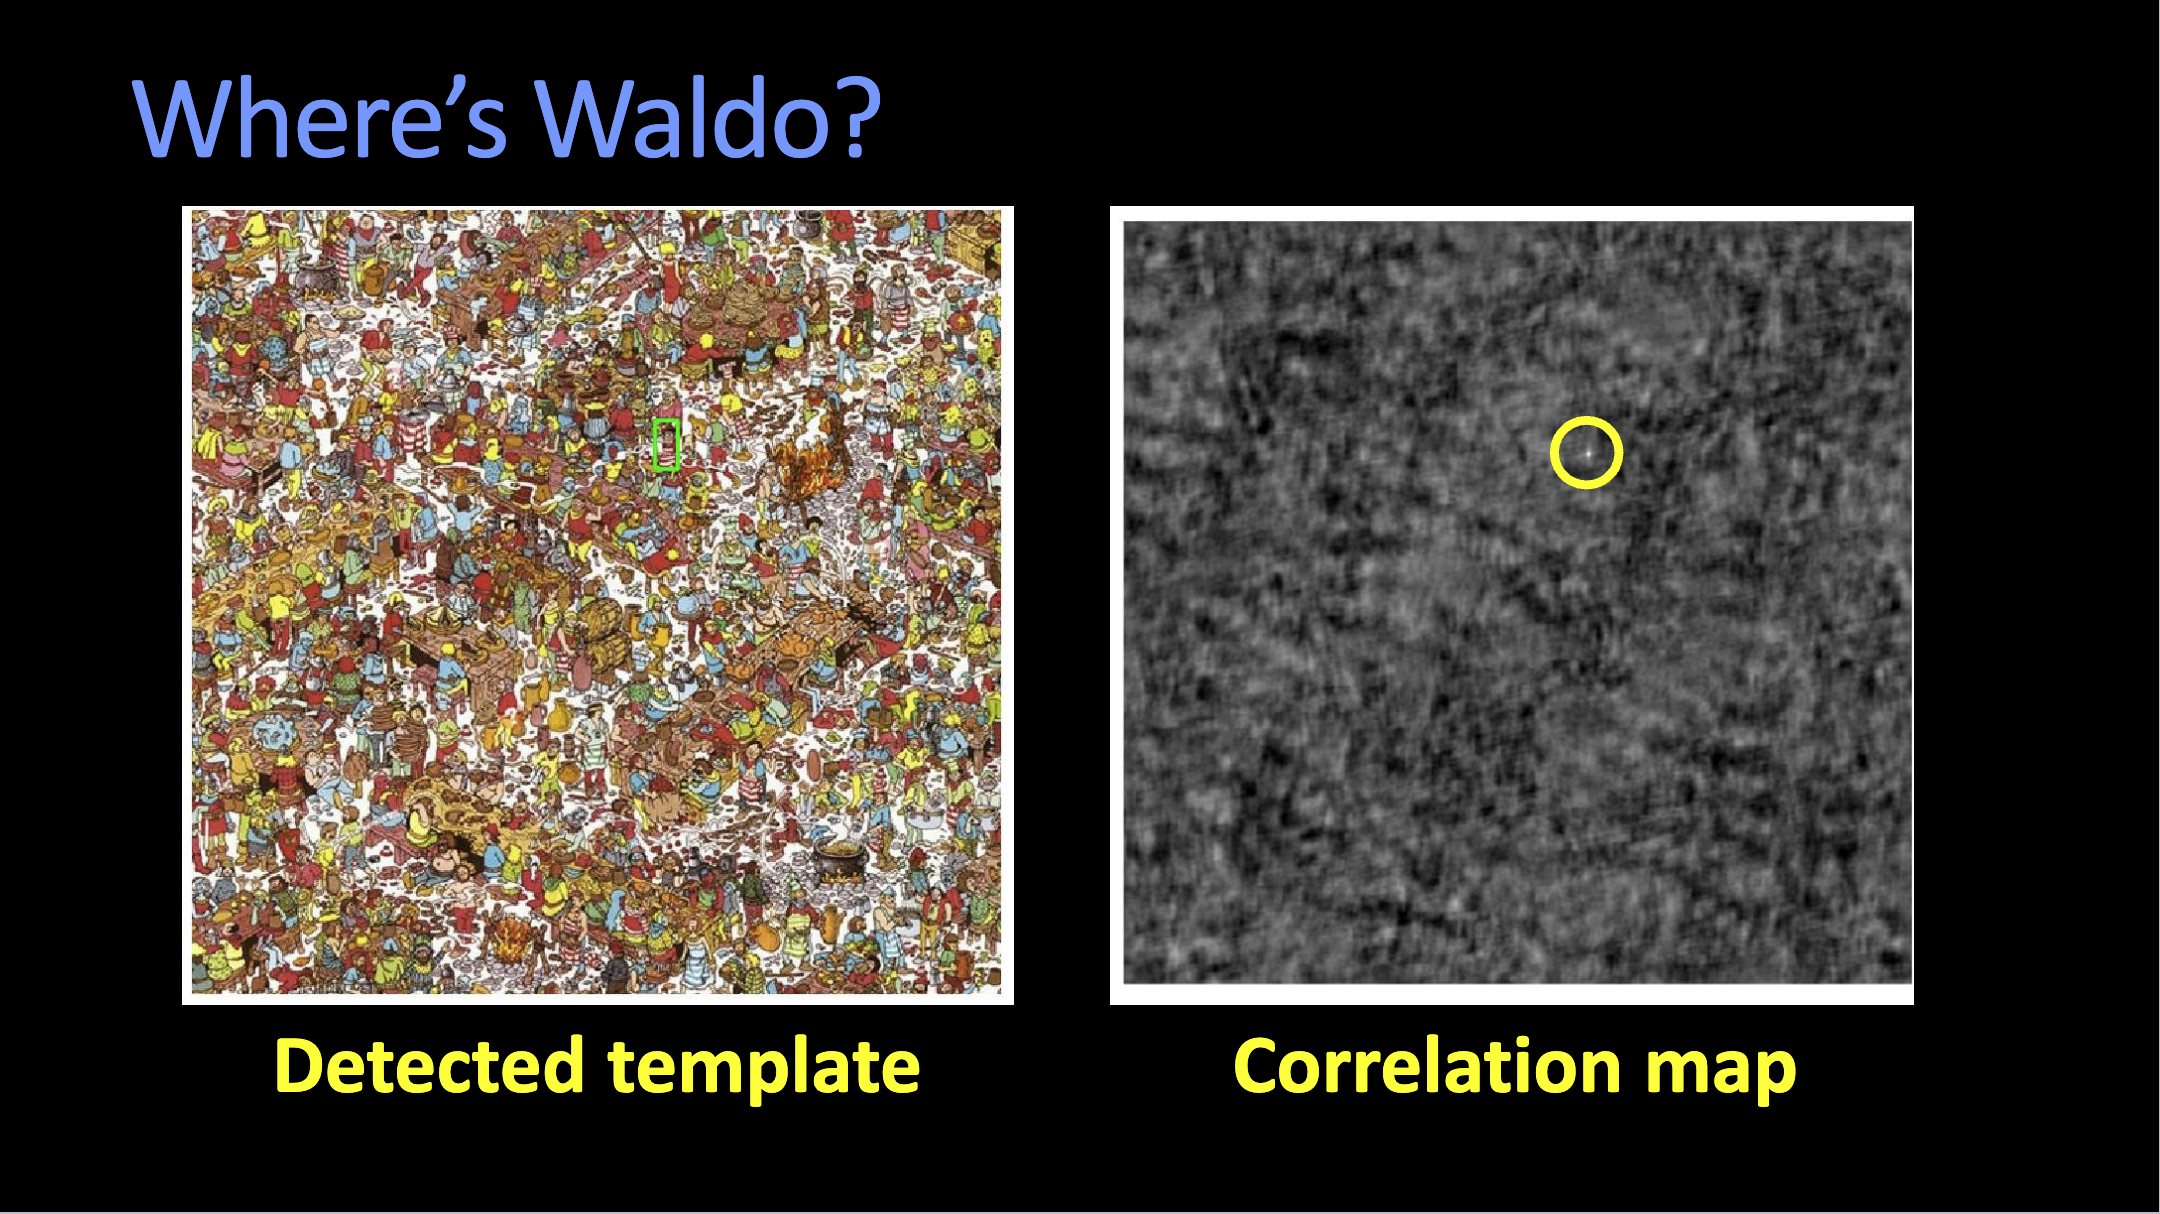
\includegraphics[width = 0.8\textwidth, trim = 0 1em 1em 0, clip]{Figures/template-match-sol.png}
    




    \begin{flushleft}
        \tiny Source: \href{https://omscs.gatech.edu/cs-6476-computer-vision}{GaTech Computer Vision}
    \end{flushleft}
    
\end{frame}



%%%%%%%%%%%%%%%%%%%%%%%%%%%%%%%%%%%%%%%

\begin{frame}{TEMPLATE MATCHING - cross correlation}

\centering
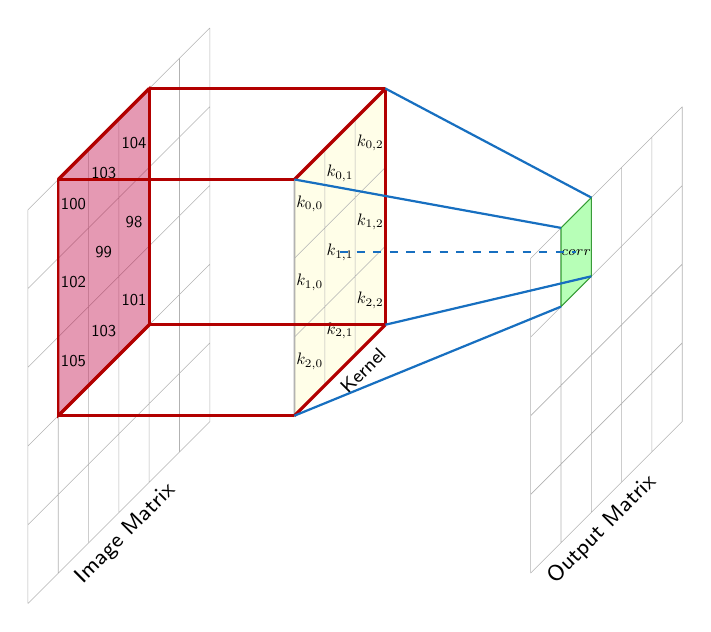
\begin{tikzpicture}[
    scale=1,
    grid line/.style={gray!60, very thin},
    matrix label/.style={font=\sffamily\bfseries},
    plane label/.style={matrix label, rotate=45, anchor=north west}
]

\tikzset{val/.style={scale=0.6, inner sep=0pt}}

% --- 1. Image Matrix ---
\begin{scope}[canvas is yz plane at x=0]
    \draw[grid line] (0,0) grid (5,6);

    \node[plane label, font=\footnotesize] at (0,5) {Image Matrix};

    % SHIFTED DOWN: was (2,3)-(5,6), now (2,2)-(5,5)
    \fill[purple, opacity=0.4] (2,2) rectangle (5,5);
    \draw[red!70!black, thick] (2,2) rectangle (5,5);

    % Values moved down by one row
    \foreach \c/\r/\val in {
        2/4/105, 3/4/102, 4/4/100,
        2/3/103, 3/3/99,  4/3/103,
        2/2/101, 3/2/98,  4/2/104
    }{
        \node[val] at (\c+0.5,\r+0.5) {\val};
    }
\end{scope}

% --- 2. Kernel Matrix ---
\begin{scope}[canvas is yz plane at x=3]
    % SHIFTED DOWN: was (2,3)-(5,6), now (2,2)-(5,5)
    \fill[yellow!10, opacity=0.9, draw=black] (2,2) rectangle (5,5);
    \draw[grid line] (2,2) grid (5,5);

    \node[plane label, font=\scriptsize] at (2,4) {Kernel};

    % Kernel values moved down
    \foreach \c/\r/\val in {
        0/2/$k_{2,0}$,  1/2/$k_{1,0}$, 2/2/$k_{0,0}$,
        0/1/$k_{2,1}$, 1/1/$k_{1,1}$,  2/1/$k_{0,1}$,
        0/0/$k_{2,2}$,  1/0/$k_{1,2}$, 2/0/$k_{0,2}$
    }{
        \node[val, text = black] at (2+\c+0.5, 2+\r+0.5) {\val};
    }

    % Highlight center weight (shifted)
    % \fill[green!20, opacity=0.8] (3,3) rectangle (4,4);
    \node[val, text = black] at (3.5,3.5) {};
\end{scope}

% --- 3. Output Matrix ---
\begin{scope}[canvas is yz plane at x=6]
    \draw[grid line] (0,0) grid (4,5);

    \node[plane label, font=\footnotesize] at (0,5) {Output Matrix};

    % Output cell stays the same visually
    \fill[green!40, opacity=0.7, draw=green!50!black] (3,3) rectangle (4,4);
    \node[scale=0.7, font = \scriptsize] at (3.5,3.5) {$corr$};
\end{scope}

% --- 4. Projection Lines (shifted down) ---
\coordinate (iTL) at (0,5,2);
\coordinate (iTR) at (0,5,5);
\coordinate (iBL) at (0,2,2);
\coordinate (iBR) at (0,2,5);

\coordinate (kTL) at (3,5,2);
\coordinate (kTR) at (3,5,5);
\coordinate (kBL) at (3,2,2);
\coordinate (kBR) at (3,2,5);

\coordinate (oTL) at (6,4,3);
\coordinate (oTR) at (6,4,4);
\coordinate (oBL) at (6,3,3);
\coordinate (oBR) at (6,3,4);


\coordinate (kC) at (3,3.5,3.5);
\coordinate (oC) at (6,3.5,3.5);

% Red prism (image -> kernel)
\begin{scope}[red!70!black, very thick]
    \draw (iTL) -- (kTL);
    \draw (iTR) -- (kTR);
    \draw (iBL) -- (kBL);
    \draw (iBR) -- (kBR);

    \draw (iTL) -- (iTR);
    \draw (kTL) -- (kTR);

    \draw (iBL) -- (iBR);
    \draw (kBL) -- (kBR);

    \draw (iTL) -- (iBL);
    \draw (kTL) -- (kBL);
\end{scope}

% Blue projection (kernel -> output)
\begin{scope}[cyan!50!blue, thick]
    \draw (kTR) -- (oTR);
    \draw (kBR) -- (oBR);
    \draw (kTL) -- (oTL);
    \draw (kBL) -- (oBL);

    \draw[dashed] (kC) -- (oC);
\end{scope}

\end{tikzpicture}

\end{frame}
%%%%%%%%%%%%%%%%%%%%%%%%%%%%%%%%%%%%%%%



% \begin{frame}{CNNs: Data-Driven Template Matching}

% \begin{itemize}
%     \item \textbf{Convolution} is the sliding window operation.
%     \item \textbf{Kernels} are the templates.
% \end{itemize}

% \[
% (I * K)(x,y) = \sum_{u,v} I(x+u,y+v)K(u,v)
% \]

% \begin{center}
% \begin{tikzpicture}[scale=0.8]
%     % Filter visualization
%     \draw[step=0.2, gray!30, very thin] (0,0) grid (1,1);
%     \node[draw=red, thick, minimum size=0.8cm] at (0.5,0.5) {\tiny $K$};
%     \node[right=1.2cm] at (1,0.5) {\textbf{Manual (CV):} Pre-defined (e.g. Sobel)};
%     \node[right=1.2cm] at (1,0) {\textbf{Learned (CNN):} Initialized randomly, refined by Backprop};
% \end{tikzpicture}
% \end{center}

% \begin{tcolorbox}[colback=orange!5, colframe=orange, boxrule=0.5pt]
%     \centering\scriptsize\bfseries
%     Difference: We no longer design the filter; the data dictates the filter.
% \end{tcolorbox}
% \end{frame}

%%%%%%%%%%%%%%%%%%%%%%%%%%%%%%%%%%%%%%%
% \begin{frame}{Evolution into CNNs}

%     In \alert<1-2>{\textbf{classical vision}}, we hand-engineer kernels (like Sobel). \\ [1em]

    
%     \begin{itemize}
%       \item Early computer vision relied on \alert<2>{hand-crafted features}
%       \item \alert<2>{Edge detection} was one of the most successful primitives
%       \item \alert<3>{CNNs} reuse and generalize these ideas
%     \end{itemize}

%     \vspace{1.5em}
    
%     \uncover<4->{In Convolutional Neural Networks (CNNs), the network \alert<4->{\textbf{learns}} these kernels.
%     } \\ [1em]

%     \uncover<5->{\begin{itemize}
%         \item Weights are optimized via backpropagation.
%         \item CNNs did not replace classical vision $\rightarrow$ they learned it.
%     \end{itemize}}
    
%     % \vspace{1.5em}

%     % \uncover<3->{
%     % So in convolutional neural networks (CNN), a CNN layer performs the same operations as a Sobel Filter, but the weights (the values inside the kernel) are optimized via backpropagation.
%     % }

    
% \end{frame}


\begin{frame}{Evolution into CNNs}

In \alert<1>{\textbf{classical vision}}, we hand-engineer kernels. \\[1.5em]

\begin{itemize}
  \item<2->[$\checkmark$] \tikz[remember picture, baseline=(b1.base)]\node(b1){}; Early computer vision relied on \alert<2>{hand-crafted features}
  
  \item<3->[$\checkmark$] \tikz[remember picture, baseline=(b2.base)]\node(b2){}; \alert<3>{Edge detection} was one of the most successful primitives
  
  \item<4->[$\times$] \tikz[remember picture, baseline=(b3.base)]\node(b3){}; Requires \alert<4>{intense human intuition} (not end-to-end).
  
  \item<5->[$\times$] \tikz[remember picture, baseline=(b4.base)]\node(b4){}; \alert<5>{Poor scalability} to complex objects or high intra-class variation.
\end{itemize}


\vspace{2em}

\textcolor{black}{{\textbf{CNNs}} reuse and generalize these ideas} \\[1em]


\begin{itemize}
    \item[] \textcolor{black}{The network  {learns} these kernels.}
    \item[] \textcolor{black}{Weights are  {optimized via backpropagation}.}
\end{itemize}



\end{frame}




%%%%%%%%%%%%%%%%%%%%%%%%%%%%%%%%%%%%%%%%%%%%%%%%

\begin{frame}{Evolution into CNNs}

In {\textbf{classical vision}}, we hand-engineer kernels. \\[1.5em]

\begin{itemize}
  \item[\textcolor{black}{$\checkmark$}] \tikz[remember picture, baseline=(b1.base)]\node(b1){}; Early computer vision relied on  {hand-crafted features}
  
  \item[\textcolor{black}{$\checkmark$}] \tikz[remember picture, baseline=(b2.base)]\node(b2){}; {Edge detection} was one of the most successful primitives
  
  \item[\textcolor{black}{$\times$}] \tikz[remember picture, baseline=(b3.base)]\node(b3){}; Requires  {intense human intuition} (not end-to-end).
  
  \item[\textcolor{black}{$\times$}] \tikz[remember picture, baseline=(b4.base)]\node(b4){}; {Poor scalability} to complex objects or high intra-class variation.
\end{itemize}

\vspace{2em}

\uncover<2->{\alert{\textbf{CNNs}} reuse and generalize these ideas} \\[1em]

\uncover<3->{
\begin{itemize}
    \item<4-> The network \alert<4->{learns} these kernels.
    \item<5-> Weights are \alert<5->{optimized via backpropagation}.
\end{itemize}
}

% Arrow connecting first and last bullet
\begin{tikzpicture}[remember picture, overlay]
    \uncover<1->{
        \draw[->, >=stealth, red, line width=5pt, opacity=0.7] 
            ([xshift=-13.5pt,yshift=6pt]b1.north) -- ([xshift=-13.5pt,yshift=-6pt]b4.south);
    }
\end{tikzpicture}

\end{frame}




%-------------------------------------------
% \begin{frame}{Why Classical Vision Hit a Ceiling}

% \begin{itemize}
%     \item Feature design requires strong human intuition
%     \item Pipelines are not end-to-end
%     \item Poor scalability to:
%     \begin{itemize}
%         \item Large datasets
%         \item Complex objects
%         \item High intra-class variation
%     \end{itemize}
% \end{itemize}

% \end{frame}


% \begin{frame}{Evolution into CNNs \& The Classical Ceiling}

%     % --- Section 1: Classical Vision ---
%     In \alert<1>{\textbf{classical vision}}, we hand-engineer kernels. \\[1em]

%     \begin{itemize}
%       \item[-] \tikz[remember picture, baseline=(b1.base)]\node(b1){}; Early CV relied on \alert<2>{hand-crafted features}.
%       \item[-] \tikz[remember picture, baseline=(b2.base)]\node(b2){}; \alert<2>{Edge detection} was a successful primitive.
%     \end{itemize}

%     % --- Section 2: The Ceiling (Merged Content) ---
%     \uncover<3->{
%     \begin{block}{The "Ceiling" of Hand-Engineering}
%         \small
%         \begin{itemize}
%             \item Requires intense human intuition (not end-to-end).
%             \item Poor scalability to complex objects or high intra-class variation.
%         \end{itemize}
%     \end{block}
%     }

%     \vspace{1em}
    
%     % --- Section 3: Transition to CNNs ---
%     \uncover<4->{\alert{\textbf{CNNs}} reuse and generalize these ideas} \\[0.5em]

%     \uncover<5->{
%     \begin{itemize}
%         \item Instead of designing, the network \alert<6->{\textbf{learns}} these kernels.
%         \item Weights are \alert<7>{\textbf{optimized via backpropagation}}.
%     \end{itemize}
%     }

%     % --- Animation Logic ---
%     \begin{tikzpicture}[remember picture, overlay, teal!50, thick]
%         % Draws the arrow between the classical bullet points once we hit the "ceiling/transition" phase
%         \uncover<3->{
%             \draw[->, >=stealth, red, line width=4pt, opacity=0.5] 
%                 ([yshift=10pt, xshift=-11pt]b1.north) -- ([yshift=-10pt, xshift=-11pt]b2.south);
%         }
%     \end{tikzpicture}

% \end{frame}

% \begin{frame}{The Bio-Inspired Hierarchy}
% \begin{columns}
%     \begin{column}{0.4\textwidth}
%         \begin{tikzpicture}[node distance=0.6cm]
%             \node[draw, fill=green!5, minimum width=2.5cm] (l1) {\tiny Low: Edges/Lines};
%             \node[draw, fill=blue!5, minimum width=2.5cm, below=of l1] (l2) {\tiny Mid: Textures/Shapes};
%             \node[draw, fill=red!5, minimum width=2.5cm, below=of l2] (l3) {\tiny High: Object Parts};
%             \draw[Stealth-, thick] (l1) -- (l2);
%             \draw[Stealth-, thick] (l2) -- (l3);
%         \end{tikzpicture}
%     \end{column}
%     \begin{column}{0.55\textwidth}
%         \scriptsize
%         \textbf{End-to-End Optimization:}
%         \begin{itemize}
%             \item \textbf{Early Layers:} Capture "What is there?" (Edges).
%             \item \textbf{Deep Layers:} Capture "What object is it?" (Semantics).
%         \end{itemize}
%         \vspace{0.2cm}
%         \textit{Classical CV tried to build this manually; CNNs do it through Stochastic Gradient Descent.}
%     \end{column}
% \end{columns}
% \end{frame}


% \input{nn-4}
% \input{nn-5}

\begin{frame}{A Simple Neural Network}

\begin{center}
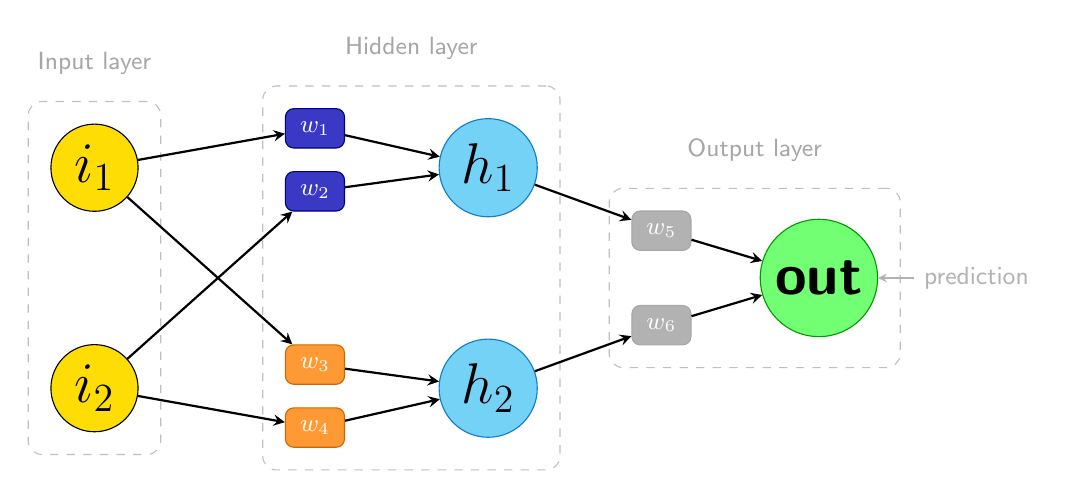
\begin{tikzpicture}[
    >=stealth,
    node distance=0cm,
    inputnode/.style={circle, draw, fill=yellow!80!orange, minimum size=1.1cm, font=\bfseries\huge},
    hiddennode/.style={circle, draw=cyan!60!blue, fill=cyan!55, minimum size=1.1cm, font=\bfseries\huge},
    outputnode/.style={circle, draw=green!60!black, fill=green!55, minimum size=1.1cm, font=\bfseries\huge},
    weightblue/.style={rectangle, rounded corners=3pt, draw=blue!50!black, fill=blue!55!gray, text=white, minimum width=0.75cm, minimum height=0.5cm, font=\bfseries\small},
    weightorange/.style={rectangle, rounded corners=3pt, draw=orange!80!black, fill=orange!80, text=white, minimum width=0.75cm, minimum height=0.5cm, font=\bfseries\small},
    weightgray/.style={rectangle, rounded corners=3pt, draw=gray!70, fill=gray!60, text=white, minimum width=0.75cm, minimum height=0.5cm, font=\bfseries\small},
    layerlabel/.style={font=\small, text=gray!70},
    dashedbox/.style={draw=gray!50, dashed, rounded corners=5pt, inner sep=8pt}
]

% Input nodes
\node[inputnode] (i1) at (0, 1.4) {$i_1$};
\node[inputnode] (i2) at (0,-1.4) {$i_2$};

% Weight boxes for h1 (blue)
\node[weightblue] (w1) at (2.8, 1.9) {$w_1$};
\node[weightblue] (w2) at (2.8, 1.1) {$w_2$};

% Weight boxes for h2 (orange)
\node[weightorange] (w3) at (2.8,-1.1) {$w_3$};
\node[weightorange] (w4) at (2.8,-1.9) {$w_4$};

% Hidden nodes
\node[hiddennode] (h1) at (5.0, 1.4) {$h_1$};
\node[hiddennode] (h2) at (5.0,-1.4) {$h_2$};

% Weights for output (gray)
\node[weightgray] (w5) at (7.2, 0.6) {$w_5$};
\node[weightgray] (w6) at (7.2,-0.6) {$w_6$};

% Output node
\node[outputnode] (out) at (9.2, 0) {\textbf{out}};

% Arrows: inputs -> weight boxes
\draw[->, thick] (i1) -- (w1);
\draw[->, thick] (i1) -- (w3);
\draw[->, thick] (i2) -- (w2);
\draw[->, thick] (i2) -- (w4);

% Arrows: weight boxes -> hidden nodes
\draw[->, thick] (w1) -- (h1);
\draw[->, thick] (w2) -- (h1);
\draw[->, thick] (w3) -- (h2);
\draw[->, thick] (w4) -- (h2);

% Arrows: hidden -> weight boxes
\draw[->, thick] (h1) -- (w5);
\draw[->, thick] (h2) -- (w6);

% Arrows: weight boxes -> output
\draw[->, thick] (w5) -- (out);
\draw[->, thick] (w6) -- (out);

% Prediction label
\node[font=\small, text=gray!60] (pred) at (11.2, 0) {prediction};
\draw[->, gray!60] (pred.west) -- (out.east);

% Dashed bounding boxes
\begin{scope}[on background layer]
  \node[dashedbox, fit=(i1)(i2)] (inputbox) {};
  \node[dashedbox, fit=(w1)(w2)(w3)(w4)(h1)(h2)] (hiddenbox) {};
  \node[dashedbox, fit=(w5)(w6)(out)] (outputbox) {};
\end{scope}

% Layer labels
\node[layerlabel, above=6pt of inputbox.north] {Input layer};
\node[layerlabel, above=6pt of hiddenbox.north] {Hidden layer};
\node[layerlabel, above=6pt of outputbox.north] {Output layer};

\end{tikzpicture}
\end{center}

\end{frame}

%~~~~~~~~~~~~~~~~~~~~~~~~~~~~~~~~~~~~~~~~~~~~~~~~~~~~~~~~~~~~~~~~~~~~~~~~~~~~~~
% \begin{frame}{From Prediction to Learning}

% \noindent\begin{minipage}[t]{0.6\textwidth}

% \textbf{prediction} $=$ {\color{green!60!black}\textbf{out}}

% \vspace{0.1cm}
% {\color{gray}$\downarrow$}
% \vspace{0.05cm}

% \noindent\begin{minipage}[c]{0.6\linewidth}
% \textbf{prediction} $= {\color{cyan!70!blue}(h_1)} w_5 + {\color{cyan!70!blue}(h_2)} w_6$
% \end{minipage}%
% \begin{minipage}[c]{0.43\linewidth}
% \vspace{2cm}
% \begin{tikzpicture}
%   \node[draw=gray!50, dashed, rounded corners=4pt, inner sep=5pt,
%         font=\scriptsize, align=left, text width=2.6cm] at (0,0) {
%     ${\color{cyan!70!blue}h_1} = {\color{orange!80!black}i_1}\,w_1 + {\color{orange!80!black}i_2}\,w_2$\\
%     ${\color{cyan!70!blue}h_2} = {\color{orange!80!black}i_1}\,w_3 + {\color{orange!80!black}i_2}\,w_4$
%   };
% \end{tikzpicture}
% \end{minipage}

% \vspace{0.15cm}
% {\color{gray}$\downarrow$}
% \vspace{0.05cm}

% {\small\textbf{prediction} $=$
%   $({\color{orange!80!black}i_1}\,\boldsymbol{w_1} + {\color{orange!80!black}i_2}\,\boldsymbol{w_2})\,w_5$
%   $+\,({\color{orange!80!black}i_1}\,\boldsymbol{w_3} + {\color{orange!80!black}i_2}\,\boldsymbol{w_4})\,w_6$}

% \vspace{0.3cm}
% \colorbox{yellow}{\parbox{0.92\linewidth}{\small to change \textit{\textbf{prediction}} value,\\
% we need to change \textbf{weights}}}

% \end{minipage}%
% \hfill
% \begin{minipage}[t]{0.38\textwidth}

% \vspace{0.8cm}
% \centering

% {\small\textit{To update weights:}}

% \vspace{0.4cm}

% $\displaystyle {}^{*\!}W_x = W_x - {\color{orange!80!black}\mathbf{a}}\!\left(\frac{\partial \mathbf{Error}}{\partial W_x}\right)$

% \vspace{0.5cm}

% \begin{tikzpicture}[>=stealth, font=\scriptsize]
%   \node[text=gray, align=center] (deriv) at (0, 0) {Derivative of Error\\with respect to weight};
%   \draw[->, gray, thin] (deriv.south) -- ++(0,-0.6);
%   \node[text=gray, align=center] at (0,-1.1) {\scriptsize$\dfrac{\partial \mathbf{Error}}{\partial W_x}$};
% \end{tikzpicture}

% \end{minipage}

% \end{frame}


% \begin{frame}{From Prediction to Learning}

% \noindent
% \begin{minipage}[t]{0.6\textwidth}

% \textbf{prediction} $=$ {\color{green!60!black}\textbf{out}}

% \vspace{0.1cm}

% {\color{gray}$\downarrow$}

% \vspace{0.08cm}

% \noindent
% \begin{minipage}[t]{0.72\linewidth}
% \textbf{prediction} \(= {\color{cyan!70!blue}(h_1)} w_5 + {\color{cyan!70!blue}(h_2)} w_6\)
% \end{minipage}%
% \vspace{2cm}
% \begin{minipage}[t]{0.24\linewidth}
% \begin{tikzpicture}[xshift=1cm]
%   \node[
%     draw=gray!50,
%     dashed,
%     rounded corners=4pt,
%     inner sep=5pt,
%     font=\scriptsize,
%     align=left,
%     text width=2.35cm
%   ] at (0,0) {
%     ${\color{cyan!70!blue}h_1} = {\color{orange!80!black}i_1}\,w_1 + {\color{orange!80!black}i_2}\,w_2$\\
%     ${\color{cyan!70!blue}h_2} = {\color{orange!80!black}i_1}\,w_3 + {\color{orange!80!black}i_2}\,w_4$
%   };
% \end{tikzpicture}
% \end{minipage}

% \vspace{0.2cm}

% {\color{gray}$\downarrow$}

% \vspace{0.08cm}

% {\small
% \textbf{prediction} \(=
% ({\color{orange!80!black}i_1}\,\boldsymbol{w_1} + {\color{orange!80!black}i_2}\,\boldsymbol{w_2})\,w_5
% + ({\color{orange!80!black}i_1}\,\boldsymbol{w_3} + {\color{orange!80!black}i_2}\,\boldsymbol{w_4})\,w_6
% \)
% }

% \vspace{1cm}

% % \colorbox{yellow!90}{%
% %   \parbox{0.92\linewidth}{%
% %     \color{black}\small
% %     to change \textit{\textbf{prediction}} value,\\
% %     we need to change {\color{red!70!black}\textbf{weights}}
% %   }%
% % }

% \colorbox{yellow!90}{%
%   \parbox{0.92\linewidth}{%
%     \color{black}\small
%     \raggedright to change \textit{\textbf{prediction}} value\\
%     \hfill we need to change {\color{red!70!black}\textbf{weights}}
%   }%
% }

% \end{minipage}%
% \hfill
% \begin{minipage}[t]{0.38\textwidth}

% \vspace{0.8cm}
% \centering

% {\small\textit{To update weights:}}

% \vspace{0.4cm}

% $\displaystyle {}^{*\!}W_x = W_x - {\color{orange!80!black}\mathbf{a}}\!\left(\frac{\partial \mathbf{Error}}{\partial W_x}\right)$

% \vspace{0.5cm}

% \begin{tikzpicture}[>=stealth, font=\scriptsize]
%   \node[text=gray, align=center] (deriv) at (0, 0)
%     {Derivative of Error\\with respect to weight};
%   \draw[->, gray, thin] (deriv.south) -- ++(0,-0.6);
%   \node[text=gray, align=center] at (0,-1.1)
%     {\scriptsize$\dfrac{\partial \mathbf{Error}}{\partial W_x}$};
% \end{tikzpicture}

% \end{minipage}

% \end{frame}

\begin{frame}{From Prediction to Learning}

\begin{columns}[T,onlytextwidth]

\column{0.62\textwidth}

\only<1->{\textbf{prediction} $=$ {\color{green!60!black}\textbf{out}}}

\vspace{0.5cm}
\only<2->{{\color{gray}$\downarrow$}}

\vspace{0.5cm}

\only<2->{
\textbf{prediction} \(= {\color{cyan!70!blue}(h_1)} w_5 + {\color{cyan!70!blue}(h_2)} w_6\)
}

\vspace{0.5cm}

\only<3->{
{\color{gray}$\downarrow$}\hspace{0.3cm}%
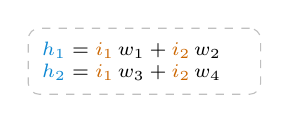
\begin{tikzpicture}[baseline=(current bounding box.center)]
  \node[
    draw=gray!50,
    dashed,
    rounded corners=4pt,
    inner sep=5pt,
    font=\scriptsize,
    align=left,
    text width=2.6cm
  ] {
    ${\color{cyan!70!blue}h_1} = {\color{orange!80!black}i_1}\,w_1 + {\color{orange!80!black}i_2}\,w_2$\\
    ${\color{cyan!70!blue}h_2} = {\color{orange!80!black}i_1}\,w_3 + {\color{orange!80!black}i_2}\,w_4$
  };
\end{tikzpicture}
}

\vspace{0.5cm}

\only<4->{
{\small
\textbf{prediction} \(=
({\color{orange!80!black}i_1}\,\boldsymbol{w_1} + {\color{orange!80!black}i_2}\,\boldsymbol{w_2})\,w_5
+ ({\color{orange!80!black}i_1}\,\boldsymbol{w_3} + {\color{orange!80!black}i_2}\,\boldsymbol{w_4})\,w_6
\)
}
}

\vspace{1cm}

\only<5->{
\colorbox{yellow!90}{%
  \parbox{0.92\linewidth}{%
    \color{black}\small
    {\raggedright to change \textit{\textbf{prediction}} value\par}
    {\raggedleft we need to change {\color{red!70!black}\textbf{weights}}\par}
  }%
}
}

\column{0.38\textwidth}

\vspace{0.8cm}
\centering

\only<6->{
{\small\textit{To update weights:}}

\vspace{0.4cm}

$\displaystyle W_x = W_x - {\color{orange!80!black}\mathbf{a}}\!\left(\frac{\partial \mathbf{Error}}{\partial W_x}\right)$
}

\vspace{0.5cm}

\only<7->{
\begin{tikzpicture}[>=stealth, font=\scriptsize]
  \node[text=gray, align=center] (deriv)
  {Derivative of Error\\with respect to weight};
  \draw[->, gray, thin] (deriv.south) -- ++(0,-0.6);
  \node[text=gray, align=center] at (0,-1.1)
  {\scriptsize$\dfrac{\partial \mathbf{Error}}{\partial W_x}$};
\end{tikzpicture}
}

\end{columns}

\end{frame}
%-------------------------------------------
% \begin{frame}{From Prediction to Learning}

% \begin{columns}[T,onlytextwidth]

% \column{0.62\textwidth}

% \textbf{prediction} $=$ {\color{green!60!black}\textbf{out}}

% \vspace{0.5cm}
% {\color{gray}$\downarrow$}

% \vspace{0.5cm}

% \textbf{prediction} \(= {\color{cyan!70!blue}(h_1)} w_5 + {\color{cyan!70!blue}(h_2)} w_6\)

% \vspace{0.5cm}

% {\color{gray}$\downarrow$}\hspace{0.3cm}%
% \begin{tikzpicture}[baseline=(current bounding box.center)]
%   \node[
%     draw=gray!50,
%     dashed,
%     rounded corners=4pt,
%     inner sep=5pt,
%     font=\scriptsize,
%     align=left,
%     text width=2.6cm
%   ] {
%     ${\color{cyan!70!blue}h_1} = {\color{orange!80!black}i_1}\,w_1 + {\color{orange!80!black}i_2}\,w_2$\\
%     ${\color{cyan!70!blue}h_2} = {\color{orange!80!black}i_1}\,w_3 + {\color{orange!80!black}i_2}\,w_4$
%   };
% \end{tikzpicture}

% \vspace{0.5cm}

% {\small
% \textbf{prediction} \(=
% ({\color{orange!80!black}i_1}\,\boldsymbol{w_1} + {\color{orange!80!black}i_2}\,\boldsymbol{w_2})\,w_5
% + ({\color{orange!80!black}i_1}\,\boldsymbol{w_3} + {\color{orange!80!black}i_2}\,\boldsymbol{w_4})\,w_6
% \)
% }

% \vspace{1cm}

% \colorbox{yellow!90}{%
%   \parbox{0.92\linewidth}{%
%     \color{black}\small
%     {\raggedright to change \textit{\textbf{prediction}} value\par}
%     {\raggedleft we need to change {\color{red!70!black}\textbf{weights}}\par}
%   }%
% }

% \column{0.38\textwidth}

% \vspace{0.8cm}
% \centering

% {\small\textit{To update weights:}}

% \vspace{0.4cm}

% $\displaystyle W_x = W_x - {\color{orange!80!black}\mathbf{a}}\!\left(\frac{\partial \mathbf{Error}}{\partial W_x}\right)$

% \vspace{0.5cm}

% \begin{tikzpicture}[>=stealth, font=\scriptsize]
%   \node[text=gray, align=center] (deriv)
%   {Derivative of Error\\with respect to weight};
%   \draw[->, gray, thin] (deriv.south) -- ++(0,-0.6);
%   \node[text=gray, align=center] at (0,-1.1)
%   {\scriptsize$\dfrac{\partial \mathbf{Error}}{\partial W_x}$};
% \end{tikzpicture}

% \end{columns}

% \end{frame}

%--------------------------------------------
\end{document}